\section{One Byte, Two Byte Exceptions}
\label{sec:vbbe21}

The one byte, two byte exceptions encoding, abbreviated to \textit{vbe21}, encodes a list of integers using one byte for each integer except for integers which cannot fit into one byte, known as \textit{exceptions}, which are encoded using two bytes. Rather than using a control code to mark where normal data and exceptions occur as in the Stream VByte codec (Section \ref{subsubsec:svb}), the exceptions are encoded at the beginning since it is expected that exceptions will occur with small probability.

The number of exceptions is written using 2 bytes, followed by the exceptions' positions in the list using 4 bytes each and the exceptions themselves using 2 bytes each.

Now, consider applying the zig-zag delta encoding to a read and then compressing using encoding $A$. Let $C_A:\Omega\to\mathbb{N}_0$ be a random variable measuring the resulting compressed size in bytes where $\Omega$ is the space of reads. Then
\begin{align*}
	C_{vbe21} &= 2 + 6X + (N - X)\\
	&= 2 + 5X + N
\end{align*}
where $N$ and $X$ are random variables measuring the read length and number of exceptions respectively.
Recall from Section \ref{subsec:prob} that the probability that a data point is greater than 255 and therefore outside the one byte range is $\sim 5\times 10^{-5}$. Thus, the expected number of exceptions is
\[ E[X] = (5 \times 10^{-5})E[N] \]
%Also, the read lengths can be modelled by the Gamma distribution $\Gamma(1.0885,0.0096)$.
where the expected read length is
\[ E[N] = 113471.4 \]
from Table \ref{tab:n}.
Then, the expected compressed size is given by
\begin{align*}
	E[C_{vbe21}] &= 2 + (2.5\times 10^{-4})E[N]+ E[N]\\
	&= 2 + 1.00025E[N]\\
	&\approx 113502.
\end{align*}
In comparison, using the Stream VByte 16 (or \textit{svb16}) encoding, the compressed size is given by
\begin{align*}
	C_{svb16} &= \lceil N/8 \rceil + 2X + (N - X)\\
	&= \lceil N/8 \rceil + X + N.
\end{align*}
Then, the expected compressed size is
\begin{align*}
	E[C_{svb16}] &= \lceil E[N]/8 \rceil + (5 \times 10^{-5})E[N] + E[N]\\
	&= \lceil E[N]/8 \rceil + 1.00005E[N]\\
	&\approx 127661\\
	&> E[C_{vbe21}].
\end{align*}
So it is clear that \textit{vbe21} saves more space than \textit{svb16}: roughly 14 KiB on average per read or an estimated 6.6 GiB for the whole data set. This is actually a very accurate estimation; see Figure \ref{fig:svb-vbe21-zd-size}.

\begin{figure}
	\centering
% Created by tikzDevice version 0.12.3.1 on 2022-10-12 10:36:34
% !TEX encoding = UTF-8 Unicode
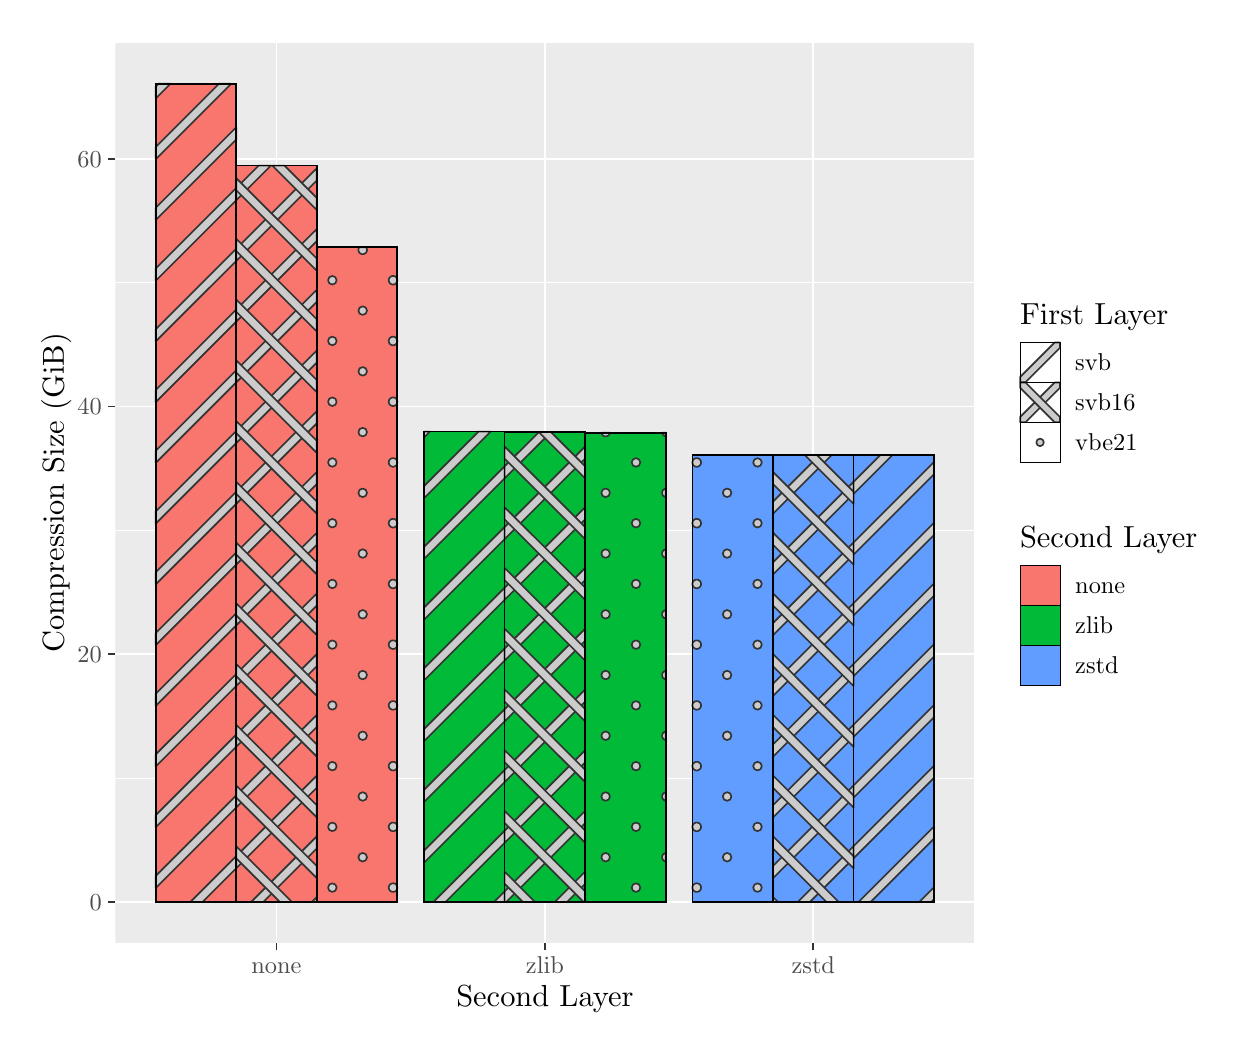
\begin{tikzpicture}[x=1pt,y=1pt]
\definecolor{fillColor}{RGB}{255,255,255}
\path[use as bounding box,fill=fillColor,fill opacity=0.00] (0,0) rectangle (433.62,361.35);
\begin{scope}
\path[clip] (  0.00,  0.00) rectangle (433.62,361.35);
\definecolor{drawColor}{RGB}{255,255,255}
\definecolor{fillColor}{RGB}{255,255,255}

\path[draw=drawColor,line width= 0.6pt,line join=round,line cap=round,fill=fillColor] (  0.00,  0.00) rectangle (433.62,361.35);
\end{scope}
\begin{scope}
\path[clip] ( 31.71, 30.69) rectangle (342.09,355.85);
\definecolor{fillColor}{gray}{0.92}

\path[fill=fillColor] ( 31.71, 30.69) rectangle (342.09,355.85);
\definecolor{drawColor}{RGB}{255,255,255}

\path[draw=drawColor,line width= 0.3pt,line join=round] ( 31.71, 90.22) --
	(342.09, 90.22);

\path[draw=drawColor,line width= 0.3pt,line join=round] ( 31.71,179.73) --
	(342.09,179.73);

\path[draw=drawColor,line width= 0.3pt,line join=round] ( 31.71,269.23) --
	(342.09,269.23);

\path[draw=drawColor,line width= 0.6pt,line join=round] ( 31.71, 45.47) --
	(342.09, 45.47);

\path[draw=drawColor,line width= 0.6pt,line join=round] ( 31.71,134.97) --
	(342.09,134.97);

\path[draw=drawColor,line width= 0.6pt,line join=round] ( 31.71,224.48) --
	(342.09,224.48);

\path[draw=drawColor,line width= 0.6pt,line join=round] ( 31.71,313.99) --
	(342.09,313.99);

\path[draw=drawColor,line width= 0.6pt,line join=round] ( 89.91, 30.69) --
	( 89.91,355.85);

\path[draw=drawColor,line width= 0.6pt,line join=round] (186.90, 30.69) --
	(186.90,355.85);

\path[draw=drawColor,line width= 0.6pt,line join=round] (283.89, 30.69) --
	(283.89,355.85);
\definecolor{fillColor}{RGB}{248,118,109}

\path[fill=fillColor] ( 46.26, 45.47) rectangle ( 75.36,341.07);

\path[fill=fillColor] ( 75.36, 45.47) rectangle (104.46,311.51);

\path[fill=fillColor] (104.46, 45.47) rectangle (133.56,282.00);
\definecolor{fillColor}{RGB}{97,156,255}

\path[fill=fillColor] (240.25, 45.47) rectangle (269.35,206.99);

\path[fill=fillColor] (269.35, 45.47) rectangle (298.44,206.97);

\path[fill=fillColor] (298.44, 45.47) rectangle (327.54,206.97);
\definecolor{fillColor}{RGB}{0,186,56}

\path[fill=fillColor] (143.25, 45.47) rectangle (172.35,215.38);

\path[fill=fillColor] (172.35, 45.47) rectangle (201.45,215.21);

\path[fill=fillColor] (201.45, 45.47) rectangle (230.55,214.96);
\definecolor{drawColor}{gray}{0.20}
\definecolor{fillColor}{gray}{0.80}

\path[draw=drawColor,line width= 0.6pt,line join=round,line cap=rect,fill=fillColor] ( 58.85, 45.47) --
	( 75.36, 61.97) --
	( 75.36, 57.58) --
	( 63.24, 45.47) --
	( 58.85, 45.47) --
	cycle;

\path[draw=drawColor,line width= 0.6pt,line join=round,line cap=rect,fill=fillColor] ( 46.26, 54.82) --
	( 75.36, 83.92) --
	( 75.36, 79.53) --
	( 46.26, 50.43) --
	( 46.26, 54.82) --
	cycle;

\path[draw=drawColor,line width= 0.6pt,line join=round,line cap=rect,fill=fillColor] ( 46.26, 76.77) --
	( 75.36,105.87) --
	( 75.36,101.48) --
	( 46.26, 72.38) --
	( 46.26, 76.77) --
	cycle;

\path[draw=drawColor,line width= 0.6pt,line join=round,line cap=rect,fill=fillColor] ( 46.26, 98.72) --
	( 75.36,127.81) --
	( 75.36,123.43) --
	( 46.26, 94.33) --
	( 46.26, 98.72) --
	cycle;

\path[draw=drawColor,line width= 0.6pt,line join=round,line cap=rect,fill=fillColor] ( 46.26,120.66) --
	( 75.36,149.76) --
	( 75.36,145.37) --
	( 46.26,116.27) --
	( 46.26,120.66) --
	cycle;

\path[draw=drawColor,line width= 0.6pt,line join=round,line cap=rect,fill=fillColor] ( 46.26,142.61) --
	( 75.36,171.71) --
	( 75.36,167.32) --
	( 46.26,138.22) --
	( 46.26,142.61) --
	cycle;

\path[draw=drawColor,line width= 0.6pt,line join=round,line cap=rect,fill=fillColor] ( 46.26,164.56) --
	( 75.36,193.66) --
	( 75.36,189.27) --
	( 46.26,160.17) --
	( 46.26,164.56) --
	cycle;

\path[draw=drawColor,line width= 0.6pt,line join=round,line cap=rect,fill=fillColor] ( 46.26,186.50) --
	( 75.36,215.60) --
	( 75.36,211.21) --
	( 46.26,182.12) --
	( 46.26,186.50) --
	cycle;

\path[draw=drawColor,line width= 0.6pt,line join=round,line cap=rect,fill=fillColor] ( 46.26,208.45) --
	( 75.36,237.55) --
	( 75.36,233.16) --
	( 46.26,204.06) --
	( 46.26,208.45) --
	cycle;

\path[draw=drawColor,line width= 0.6pt,line join=round,line cap=rect,fill=fillColor] ( 46.26,230.40) --
	( 75.36,259.50) --
	( 75.36,255.11) --
	( 46.26,226.01) --
	( 46.26,230.40) --
	cycle;

\path[draw=drawColor,line width= 0.6pt,line join=round,line cap=rect,fill=fillColor] ( 46.26,252.35) --
	( 75.36,281.44) --
	( 75.36,277.05) --
	( 46.26,247.96) --
	( 46.26,252.35) --
	cycle;

\path[draw=drawColor,line width= 0.6pt,line join=round,line cap=rect,fill=fillColor] ( 46.26,274.29) --
	( 75.36,303.39) --
	( 75.36,299.00) --
	( 46.26,269.90) --
	( 46.26,274.29) --
	cycle;

\path[draw=drawColor,line width= 0.6pt,line join=round,line cap=rect,fill=fillColor] ( 46.26,296.24) --
	( 75.36,325.34) --
	( 75.36,320.95) --
	( 46.26,291.85) --
	( 46.26,296.24) --
	cycle;

\path[draw=drawColor,line width= 0.6pt,line join=round,line cap=rect,fill=fillColor] ( 46.26,318.19) --
	( 69.14,341.07) --
	( 73.53,341.07) --
	( 46.26,313.80) --
	( 46.26,318.19) --
	cycle;

\path[draw=drawColor,line width= 0.6pt,line join=round,line cap=rect,fill=fillColor] ( 46.26,340.13) --
	( 47.20,341.07) --
	( 51.59,341.07) --
	( 46.26,335.74) --
	( 46.26,340.13) --
	cycle;

\path[draw=drawColor,line width= 0.6pt,line join=round,line cap=rect,fill=fillColor] (102.75, 45.47) --
	(104.46, 47.18) --
	(104.46, 45.47) --
	(102.75, 45.47) --
	cycle;

\path[draw=drawColor,line width= 0.6pt,line join=round,line cap=rect,fill=fillColor] ( 80.80, 45.47) --
	(104.46, 69.12) --
	(104.46, 64.73) --
	( 85.19, 45.47) --
	( 80.80, 45.47) --
	cycle;

\path[draw=drawColor,line width= 0.6pt,line join=round,line cap=rect,fill=fillColor] ( 75.36, 61.97) --
	(104.46, 91.07) --
	(104.46, 86.68) --
	( 75.36, 57.58) --
	( 75.36, 61.97) --
	cycle;

\path[draw=drawColor,line width= 0.6pt,line join=round,line cap=rect,fill=fillColor] ( 75.36, 83.92) --
	(104.46,113.02) --
	(104.46,108.63) --
	( 75.36, 79.53) --
	( 75.36, 83.92) --
	cycle;

\path[draw=drawColor,line width= 0.6pt,line join=round,line cap=rect,fill=fillColor] ( 75.36,105.87) --
	(104.46,134.97) --
	(104.46,130.58) --
	( 75.36,101.48) --
	( 75.36,105.87) --
	cycle;

\path[draw=drawColor,line width= 0.6pt,line join=round,line cap=rect,fill=fillColor] ( 75.36,127.81) --
	(104.46,156.91) --
	(104.46,152.52) --
	( 75.36,123.43) --
	( 75.36,127.81) --
	cycle;

\path[draw=drawColor,line width= 0.6pt,line join=round,line cap=rect,fill=fillColor] ( 75.36,149.76) --
	(104.46,178.86) --
	(104.46,174.47) --
	( 75.36,145.37) --
	( 75.36,149.76) --
	cycle;

\path[draw=drawColor,line width= 0.6pt,line join=round,line cap=rect,fill=fillColor] ( 75.36,171.71) --
	(104.46,200.81) --
	(104.46,196.42) --
	( 75.36,167.32) --
	( 75.36,171.71) --
	cycle;

\path[draw=drawColor,line width= 0.6pt,line join=round,line cap=rect,fill=fillColor] ( 75.36,193.66) --
	(104.46,222.75) --
	(104.46,218.36) --
	( 75.36,189.27) --
	( 75.36,193.66) --
	cycle;

\path[draw=drawColor,line width= 0.6pt,line join=round,line cap=rect,fill=fillColor] ( 75.36,215.60) --
	(104.46,244.70) --
	(104.46,240.31) --
	( 75.36,211.21) --
	( 75.36,215.60) --
	cycle;

\path[draw=drawColor,line width= 0.6pt,line join=round,line cap=rect,fill=fillColor] ( 75.36,237.55) --
	(104.46,266.65) --
	(104.46,262.26) --
	( 75.36,233.16) --
	( 75.36,237.55) --
	cycle;

\path[draw=drawColor,line width= 0.6pt,line join=round,line cap=rect,fill=fillColor] ( 75.36,259.50) --
	(104.46,288.59) --
	(104.46,284.21) --
	( 75.36,255.11) --
	( 75.36,259.50) --
	cycle;

\path[draw=drawColor,line width= 0.6pt,line join=round,line cap=rect,fill=fillColor] ( 75.36,281.44) --
	(104.46,310.54) --
	(104.46,306.15) --
	( 75.36,277.05) --
	( 75.36,281.44) --
	cycle;

\path[draw=drawColor,line width= 0.6pt,line join=round,line cap=rect,fill=fillColor] ( 75.36,303.39) --
	( 83.48,311.51) --
	( 87.87,311.51) --
	( 75.36,299.00) --
	( 75.36,303.39) --
	cycle;

\path[draw=drawColor,line width= 0.6pt,line join=round,line cap=rect,fill=fillColor] ( 75.36, 65.59) --
	( 95.48, 45.47) --
	( 91.09, 45.47) --
	( 75.36, 61.20) --
	( 75.36, 65.59) --
	cycle;

\path[draw=drawColor,line width= 0.6pt,line join=round,line cap=rect,fill=fillColor] ( 75.36, 87.53) --
	(104.46, 58.44) --
	(104.46, 54.05) --
	( 75.36, 83.14) --
	( 75.36, 87.53) --
	cycle;

\path[draw=drawColor,line width= 0.6pt,line join=round,line cap=rect,fill=fillColor] ( 75.36,109.48) --
	(104.46, 80.38) --
	(104.46, 75.99) --
	( 75.36,105.09) --
	( 75.36,109.48) --
	cycle;

\path[draw=drawColor,line width= 0.6pt,line join=round,line cap=rect,fill=fillColor] ( 75.36,131.43) --
	(104.46,102.33) --
	(104.46, 97.94) --
	( 75.36,127.04) --
	( 75.36,131.43) --
	cycle;

\path[draw=drawColor,line width= 0.6pt,line join=round,line cap=rect,fill=fillColor] ( 75.36,153.38) --
	(104.46,124.28) --
	(104.46,119.89) --
	( 75.36,148.99) --
	( 75.36,153.38) --
	cycle;

\path[draw=drawColor,line width= 0.6pt,line join=round,line cap=rect,fill=fillColor] ( 75.36,175.32) --
	(104.46,146.22) --
	(104.46,141.84) --
	( 75.36,170.93) --
	( 75.36,175.32) --
	cycle;

\path[draw=drawColor,line width= 0.6pt,line join=round,line cap=rect,fill=fillColor] ( 75.36,197.27) --
	(104.46,168.17) --
	(104.46,163.78) --
	( 75.36,192.88) --
	( 75.36,197.27) --
	cycle;

\path[draw=drawColor,line width= 0.6pt,line join=round,line cap=rect,fill=fillColor] ( 75.36,219.22) --
	(104.46,190.12) --
	(104.46,185.73) --
	( 75.36,214.83) --
	( 75.36,219.22) --
	cycle;

\path[draw=drawColor,line width= 0.6pt,line join=round,line cap=rect,fill=fillColor] ( 75.36,241.16) --
	(104.46,212.07) --
	(104.46,207.68) --
	( 75.36,236.77) --
	( 75.36,241.16) --
	cycle;

\path[draw=drawColor,line width= 0.6pt,line join=round,line cap=rect,fill=fillColor] ( 75.36,263.11) --
	(104.46,234.01) --
	(104.46,229.62) --
	( 75.36,258.72) --
	( 75.36,263.11) --
	cycle;

\path[draw=drawColor,line width= 0.6pt,line join=round,line cap=rect,fill=fillColor] ( 75.36,285.06) --
	(104.46,255.96) --
	(104.46,251.57) --
	( 75.36,280.67) --
	( 75.36,285.06) --
	cycle;

\path[draw=drawColor,line width= 0.6pt,line join=round,line cap=rect,fill=fillColor] ( 75.36,307.00) --
	(104.46,277.91) --
	(104.46,273.52) --
	( 75.36,302.62) --
	( 75.36,307.00) --
	cycle;

\path[draw=drawColor,line width= 0.6pt,line join=round,line cap=rect,fill=fillColor] ( 92.80,311.51) --
	(104.46,299.85) --
	(104.46,295.46) --
	( 88.41,311.51) --
	( 92.80,311.51) --
	cycle;

\path[draw=drawColor,line width= 0.6pt,line join=round,line cap=round,fill=fillColor] (110.09, 94.51) circle (  1.55);

\path[draw=drawColor,line width= 0.6pt,line join=round,line cap=round,fill=fillColor] (110.09,116.45) circle (  1.55);

\path[draw=drawColor,line width= 0.6pt,line join=round,line cap=round,fill=fillColor] (110.09,138.40) circle (  1.55);

\path[draw=drawColor,line width= 0.6pt,line join=round,line cap=round,fill=fillColor] (110.09,226.19) circle (  1.55);

\path[draw=drawColor,line width= 0.6pt,line join=round,line cap=round,fill=fillColor] (110.09,248.14) circle (  1.55);

\path[draw=drawColor,line width= 0.6pt,line join=round,line cap=round,fill=fillColor] (110.09,160.35) circle (  1.55);

\path[draw=drawColor,line width= 0.6pt,line join=round,line cap=round,fill=fillColor] (110.09,204.24) circle (  1.55);

\path[draw=drawColor,line width= 0.6pt,line join=round,line cap=round,fill=fillColor] (110.09,182.29) circle (  1.55);

\path[draw=drawColor,line width= 0.6pt,line join=round,line cap=round,fill=fillColor] (110.09,270.08) circle (  1.55);

\path[draw=drawColor,line width= 0.6pt,line join=round,line cap=round,fill=fillColor] (110.09, 50.61) circle (  1.55);

\path[draw=drawColor,line width= 0.6pt,line join=round,line cap=round,fill=fillColor] (110.09, 72.56) circle (  1.55);

\path[draw=drawColor,line width= 0.6pt,line join=round,line cap=round,fill=fillColor] (121.06,127.43) circle (  1.55);

\path[draw=drawColor,line width= 0.6pt,line join=round,line cap=round,fill=fillColor] (121.06,149.37) circle (  1.55);

\path[draw=drawColor,line width= 0.6pt,line join=round,line cap=round,fill=fillColor] (121.06,237.16) circle (  1.55);

\path[draw=drawColor,line width= 0.6pt,line join=round,line cap=round,fill=fillColor] (121.06,105.48) circle (  1.55);

\path[draw=drawColor,line width= 0.6pt,line join=round,line cap=round,fill=fillColor] (121.06,171.32) circle (  1.55);

\path[draw=drawColor,line width= 0.6pt,line join=round,line cap=round,fill=fillColor] (121.06,193.27) circle (  1.55);

\path[draw=drawColor,line width= 0.6pt,line join=round,line cap=round,fill=fillColor] (121.06,215.21) circle (  1.55);

\path[draw=drawColor,line width= 0.6pt,line join=round,line cap=round,fill=fillColor] (121.06,259.11) circle (  1.55);

\path[draw=drawColor,line width= 0.6pt,line join=round,line cap=round,fill=fillColor] (121.06, 83.53) circle (  1.55);

\path[draw=drawColor,line width= 0.6pt,line join=round,line cap=round,fill=fillColor] (121.06, 61.59) circle (  1.55);

\path[draw=drawColor,line width= 0.6pt,line join=round,line cap=round,fill=fillColor] (122.30,282.00) --
	(122.34,281.93) --
	(122.40,281.85) --
	(122.44,281.76) --
	(122.48,281.67) --
	(122.52,281.58) --
	(122.55,281.49) --
	(122.57,281.39) --
	(122.59,281.30) --
	(122.61,281.20) --
	(122.61,281.10) --
	(122.61,281.01) --
	(122.61,280.91) --
	(122.59,280.81) --
	(122.57,280.72) --
	(122.55,280.62) --
	(122.52,280.53) --
	(122.48,280.44) --
	(122.44,280.35) --
	(122.40,280.27) --
	(122.34,280.18) --
	(122.29,280.11) --
	(122.22,280.03) --
	(122.16,279.96) --
	(122.09,279.89) --
	(122.01,279.83) --
	(121.93,279.77) --
	(121.85,279.72) --
	(121.76,279.67) --
	(121.68,279.63) --
	(121.59,279.60) --
	(121.49,279.57) --
	(121.40,279.54) --
	(121.30,279.52) --
	(121.21,279.51) --
	(121.11,279.51) --
	(121.01,279.51) --
	(120.91,279.51) --
	(120.82,279.52) --
	(120.72,279.54) --
	(120.63,279.57) --
	(120.53,279.60) --
	(120.44,279.63) --
	(120.36,279.67) --
	(120.27,279.72) --
	(120.19,279.77) --
	(120.11,279.83) --
	(120.03,279.89) --
	(119.96,279.96) --
	(119.90,280.03) --
	(119.83,280.11) --
	(119.78,280.18) --
	(119.72,280.27) --
	(119.68,280.35) --
	(119.64,280.44) --
	(119.60,280.53) --
	(119.57,280.62) --
	(119.55,280.72) --
	(119.53,280.81) --
	(119.52,280.91) --
	(119.51,281.01) --
	(119.51,281.10) --
	(119.52,281.20) --
	(119.53,281.30) --
	(119.55,281.39) --
	(119.57,281.49) --
	(119.60,281.58) --
	(119.64,281.67) --
	(119.68,281.76) --
	(119.72,281.85) --
	(119.78,281.93) --
	(119.83,282.00) --
	(122.30,282.00) --
	cycle;

\path[draw=drawColor,line width= 0.6pt,line join=round,line cap=round,fill=fillColor] (133.56,116.15) --
	(133.55,116.11) --
	(133.52,116.02) --
	(133.49,115.93) --
	(133.46,115.84) --
	(133.42,115.75) --
	(133.37,115.66) --
	(133.32,115.58) --
	(133.26,115.50) --
	(133.20,115.43) --
	(133.13,115.36) --
	(133.06,115.29) --
	(132.98,115.23) --
	(132.91,115.17) --
	(132.82,115.12) --
	(132.74,115.07) --
	(132.65,115.03) --
	(132.56,114.99) --
	(132.47,114.96) --
	(132.37,114.94) --
	(132.28,114.92) --
	(132.18,114.91) --
	(132.08,114.90) --
	(131.99,114.90) --
	(131.89,114.91) --
	(131.79,114.92) --
	(131.70,114.94) --
	(131.60,114.96) --
	(131.51,114.99) --
	(131.42,115.03) --
	(131.33,115.07) --
	(131.24,115.12) --
	(131.16,115.17) --
	(131.08,115.23) --
	(131.01,115.29) --
	(130.94,115.36) --
	(130.87,115.43) --
	(130.81,115.50) --
	(130.75,115.58) --
	(130.70,115.66) --
	(130.65,115.75) --
	(130.61,115.84) --
	(130.57,115.93) --
	(130.54,116.02) --
	(130.52,116.11) --
	(130.50,116.21) --
	(130.49,116.31) --
	(130.48,116.40) --
	(130.48,116.50) --
	(130.49,116.60) --
	(130.50,116.70) --
	(130.52,116.79) --
	(130.54,116.89) --
	(130.57,116.98) --
	(130.61,117.07) --
	(130.65,117.16) --
	(130.70,117.24) --
	(130.75,117.33) --
	(130.81,117.40) --
	(130.87,117.48) --
	(130.94,117.55) --
	(131.01,117.62) --
	(131.08,117.68) --
	(131.16,117.74) --
	(131.24,117.79) --
	(131.33,117.84) --
	(131.42,117.88) --
	(131.51,117.91) --
	(131.60,117.94) --
	(131.70,117.97) --
	(131.79,117.99) --
	(131.89,118.00) --
	(131.99,118.00) --
	(132.08,118.00) --
	(132.18,118.00) --
	(132.28,117.99) --
	(132.37,117.97) --
	(132.47,117.94) --
	(132.56,117.91) --
	(132.65,117.88) --
	(132.74,117.84) --
	(132.82,117.79) --
	(132.91,117.74) --
	(132.98,117.68) --
	(133.06,117.62) --
	(133.13,117.55) --
	(133.20,117.48) --
	(133.26,117.40) --
	(133.32,117.33) --
	(133.37,117.24) --
	(133.42,117.16) --
	(133.46,117.07) --
	(133.49,116.98) --
	(133.52,116.89) --
	(133.55,116.79) --
	(133.56,116.76) --
	(133.56,116.15) --
	cycle;

\path[draw=drawColor,line width= 0.6pt,line join=round,line cap=round,fill=fillColor] (133.56,138.10) --
	(133.55,138.06) --
	(133.52,137.97) --
	(133.49,137.87) --
	(133.46,137.78) --
	(133.42,137.70) --
	(133.37,137.61) --
	(133.32,137.53) --
	(133.26,137.45) --
	(133.20,137.37) --
	(133.13,137.30) --
	(133.06,137.24) --
	(132.98,137.17) --
	(132.91,137.12) --
	(132.82,137.06) --
	(132.74,137.02) --
	(132.65,136.98) --
	(132.56,136.94) --
	(132.47,136.91) --
	(132.37,136.89) --
	(132.28,136.87) --
	(132.18,136.86) --
	(132.08,136.85) --
	(131.99,136.85) --
	(131.89,136.86) --
	(131.79,136.87) --
	(131.70,136.89) --
	(131.60,136.91) --
	(131.51,136.94) --
	(131.42,136.98) --
	(131.33,137.02) --
	(131.24,137.06) --
	(131.16,137.12) --
	(131.08,137.17) --
	(131.01,137.24) --
	(130.94,137.30) --
	(130.87,137.37) --
	(130.81,137.45) --
	(130.75,137.53) --
	(130.70,137.61) --
	(130.65,137.70) --
	(130.61,137.78) --
	(130.57,137.87) --
	(130.54,137.97) --
	(130.52,138.06) --
	(130.50,138.16) --
	(130.49,138.25) --
	(130.48,138.35) --
	(130.48,138.45) --
	(130.49,138.55) --
	(130.50,138.64) --
	(130.52,138.74) --
	(130.54,138.83) --
	(130.57,138.93) --
	(130.61,139.02) --
	(130.65,139.10) --
	(130.70,139.19) --
	(130.75,139.27) --
	(130.81,139.35) --
	(130.87,139.43) --
	(130.94,139.50) --
	(131.01,139.56) --
	(131.08,139.63) --
	(131.16,139.68) --
	(131.24,139.74) --
	(131.33,139.78) --
	(131.42,139.82) --
	(131.51,139.86) --
	(131.60,139.89) --
	(131.70,139.91) --
	(131.79,139.93) --
	(131.89,139.95) --
	(131.99,139.95) --
	(132.08,139.95) --
	(132.18,139.95) --
	(132.28,139.93) --
	(132.37,139.91) --
	(132.47,139.89) --
	(132.56,139.86) --
	(132.65,139.82) --
	(132.74,139.78) --
	(132.82,139.74) --
	(132.91,139.68) --
	(132.98,139.63) --
	(133.06,139.56) --
	(133.13,139.50) --
	(133.20,139.43) --
	(133.26,139.35) --
	(133.32,139.27) --
	(133.37,139.19) --
	(133.42,139.10) --
	(133.46,139.02) --
	(133.49,138.93) --
	(133.52,138.83) --
	(133.55,138.74) --
	(133.56,138.70) --
	(133.56,138.10) --
	cycle;

\path[draw=drawColor,line width= 0.6pt,line join=round,line cap=round,fill=fillColor] (133.56,225.89) --
	(133.55,225.85) --
	(133.52,225.76) --
	(133.49,225.66) --
	(133.46,225.57) --
	(133.42,225.48) --
	(133.37,225.40) --
	(133.32,225.32) --
	(133.26,225.24) --
	(133.20,225.16) --
	(133.13,225.09) --
	(133.06,225.02) --
	(132.98,224.96) --
	(132.91,224.90) --
	(132.82,224.85) --
	(132.74,224.81) --
	(132.65,224.76) --
	(132.56,224.73) --
	(132.47,224.70) --
	(132.37,224.67) --
	(132.28,224.66) --
	(132.18,224.64) --
	(132.08,224.64) --
	(131.99,224.64) --
	(131.89,224.64) --
	(131.79,224.66) --
	(131.70,224.67) --
	(131.60,224.70) --
	(131.51,224.73) --
	(131.42,224.76) --
	(131.33,224.81) --
	(131.24,224.85) --
	(131.16,224.90) --
	(131.08,224.96) --
	(131.01,225.02) --
	(130.94,225.09) --
	(130.87,225.16) --
	(130.81,225.24) --
	(130.75,225.32) --
	(130.70,225.40) --
	(130.65,225.48) --
	(130.61,225.57) --
	(130.57,225.66) --
	(130.54,225.76) --
	(130.52,225.85) --
	(130.50,225.95) --
	(130.49,226.04) --
	(130.48,226.14) --
	(130.48,226.24) --
	(130.49,226.33) --
	(130.50,226.43) --
	(130.52,226.53) --
	(130.54,226.62) --
	(130.57,226.71) --
	(130.61,226.80) --
	(130.65,226.89) --
	(130.70,226.98) --
	(130.75,227.06) --
	(130.81,227.14) --
	(130.87,227.21) --
	(130.94,227.29) --
	(131.01,227.35) --
	(131.08,227.41) --
	(131.16,227.47) --
	(131.24,227.52) --
	(131.33,227.57) --
	(131.42,227.61) --
	(131.51,227.65) --
	(131.60,227.68) --
	(131.70,227.70) --
	(131.79,227.72) --
	(131.89,227.73) --
	(131.99,227.74) --
	(132.08,227.74) --
	(132.18,227.73) --
	(132.28,227.72) --
	(132.37,227.70) --
	(132.47,227.68) --
	(132.56,227.65) --
	(132.65,227.61) --
	(132.74,227.57) --
	(132.82,227.52) --
	(132.91,227.47) --
	(132.98,227.41) --
	(133.06,227.35) --
	(133.13,227.29) --
	(133.20,227.21) --
	(133.26,227.14) --
	(133.32,227.06) --
	(133.37,226.98) --
	(133.42,226.89) --
	(133.46,226.80) --
	(133.49,226.71) --
	(133.52,226.62) --
	(133.55,226.53) --
	(133.56,226.49) --
	(133.56,225.89) --
	cycle;

\path[draw=drawColor,line width= 0.6pt,line join=round,line cap=round,fill=fillColor] (133.56,160.04) --
	(133.55,160.01) --
	(133.52,159.91) --
	(133.49,159.82) --
	(133.46,159.73) --
	(133.42,159.64) --
	(133.37,159.56) --
	(133.32,159.47) --
	(133.26,159.40) --
	(133.20,159.32) --
	(133.13,159.25) --
	(133.06,159.18) --
	(132.98,159.12) --
	(132.91,159.06) --
	(132.82,159.01) --
	(132.74,158.96) --
	(132.65,158.92) --
	(132.56,158.89) --
	(132.47,158.86) --
	(132.37,158.83) --
	(132.28,158.81) --
	(132.18,158.80) --
	(132.08,158.80) --
	(131.99,158.80) --
	(131.89,158.80) --
	(131.79,158.81) --
	(131.70,158.83) --
	(131.60,158.86) --
	(131.51,158.89) --
	(131.42,158.92) --
	(131.33,158.96) --
	(131.24,159.01) --
	(131.16,159.06) --
	(131.08,159.12) --
	(131.01,159.18) --
	(130.94,159.25) --
	(130.87,159.32) --
	(130.81,159.40) --
	(130.75,159.47) --
	(130.70,159.56) --
	(130.65,159.64) --
	(130.61,159.73) --
	(130.57,159.82) --
	(130.54,159.91) --
	(130.52,160.01) --
	(130.50,160.10) --
	(130.49,160.20) --
	(130.48,160.30) --
	(130.48,160.40) --
	(130.49,160.49) --
	(130.50,160.59) --
	(130.52,160.69) --
	(130.54,160.78) --
	(130.57,160.87) --
	(130.61,160.96) --
	(130.65,161.05) --
	(130.70,161.14) --
	(130.75,161.22) --
	(130.81,161.30) --
	(130.87,161.37) --
	(130.94,161.44) --
	(131.01,161.51) --
	(131.08,161.57) --
	(131.16,161.63) --
	(131.24,161.68) --
	(131.33,161.73) --
	(131.42,161.77) --
	(131.51,161.81) --
	(131.60,161.84) --
	(131.70,161.86) --
	(131.79,161.88) --
	(131.89,161.89) --
	(131.99,161.90) --
	(132.08,161.90) --
	(132.18,161.89) --
	(132.28,161.88) --
	(132.37,161.86) --
	(132.47,161.84) --
	(132.56,161.81) --
	(132.65,161.77) --
	(132.74,161.73) --
	(132.82,161.68) --
	(132.91,161.63) --
	(132.98,161.57) --
	(133.06,161.51) --
	(133.13,161.44) --
	(133.20,161.37) --
	(133.26,161.30) --
	(133.32,161.22) --
	(133.37,161.14) --
	(133.42,161.05) --
	(133.46,160.96) --
	(133.49,160.87) --
	(133.52,160.78) --
	(133.55,160.69) --
	(133.56,160.65) --
	(133.56,160.04) --
	cycle;

\path[draw=drawColor,line width= 0.6pt,line join=round,line cap=round,fill=fillColor] (133.56,247.83) --
	(133.55,247.80) --
	(133.52,247.70) --
	(133.49,247.61) --
	(133.46,247.52) --
	(133.42,247.43) --
	(133.37,247.35) --
	(133.32,247.26) --
	(133.26,247.18) --
	(133.20,247.11) --
	(133.13,247.04) --
	(133.06,246.97) --
	(132.98,246.91) --
	(132.91,246.85) --
	(132.82,246.80) --
	(132.74,246.75) --
	(132.65,246.71) --
	(132.56,246.68) --
	(132.47,246.65) --
	(132.37,246.62) --
	(132.28,246.60) --
	(132.18,246.59) --
	(132.08,246.58) --
	(131.99,246.58) --
	(131.89,246.59) --
	(131.79,246.60) --
	(131.70,246.62) --
	(131.60,246.65) --
	(131.51,246.68) --
	(131.42,246.71) --
	(131.33,246.75) --
	(131.24,246.80) --
	(131.16,246.85) --
	(131.08,246.91) --
	(131.01,246.97) --
	(130.94,247.04) --
	(130.87,247.11) --
	(130.81,247.18) --
	(130.75,247.26) --
	(130.70,247.35) --
	(130.65,247.43) --
	(130.61,247.52) --
	(130.57,247.61) --
	(130.54,247.70) --
	(130.52,247.80) --
	(130.50,247.89) --
	(130.49,247.99) --
	(130.48,248.09) --
	(130.48,248.18) --
	(130.49,248.28) --
	(130.50,248.38) --
	(130.52,248.47) --
	(130.54,248.57) --
	(130.57,248.66) --
	(130.61,248.75) --
	(130.65,248.84) --
	(130.70,248.93) --
	(130.75,249.01) --
	(130.81,249.09) --
	(130.87,249.16) --
	(130.94,249.23) --
	(131.01,249.30) --
	(131.08,249.36) --
	(131.16,249.42) --
	(131.24,249.47) --
	(131.33,249.52) --
	(131.42,249.56) --
	(131.51,249.60) --
	(131.60,249.63) --
	(131.70,249.65) --
	(131.79,249.67) --
	(131.89,249.68) --
	(131.99,249.69) --
	(132.08,249.69) --
	(132.18,249.68) --
	(132.28,249.67) --
	(132.37,249.65) --
	(132.47,249.63) --
	(132.56,249.60) --
	(132.65,249.56) --
	(132.74,249.52) --
	(132.82,249.47) --
	(132.91,249.42) --
	(132.98,249.36) --
	(133.06,249.30) --
	(133.13,249.23) --
	(133.20,249.16) --
	(133.26,249.09) --
	(133.32,249.01) --
	(133.37,248.93) --
	(133.42,248.84) --
	(133.46,248.75) --
	(133.49,248.66) --
	(133.52,248.57) --
	(133.55,248.47) --
	(133.56,248.44) --
	(133.56,247.83) --
	cycle;

\path[draw=drawColor,line width= 0.6pt,line join=round,line cap=round,fill=fillColor] (133.56, 72.26) --
	(133.55, 72.22) --
	(133.52, 72.13) --
	(133.49, 72.03) --
	(133.46, 71.94) --
	(133.42, 71.85) --
	(133.37, 71.77) --
	(133.32, 71.69) --
	(133.26, 71.61) --
	(133.20, 71.53) --
	(133.13, 71.46) --
	(133.06, 71.39) --
	(132.98, 71.33) --
	(132.91, 71.28) --
	(132.82, 71.22) --
	(132.74, 71.18) --
	(132.65, 71.13) --
	(132.56, 71.10) --
	(132.47, 71.07) --
	(132.37, 71.04) --
	(132.28, 71.03) --
	(132.18, 71.01) --
	(132.08, 71.01) --
	(131.99, 71.01) --
	(131.89, 71.01) --
	(131.79, 71.03) --
	(131.70, 71.04) --
	(131.60, 71.07) --
	(131.51, 71.10) --
	(131.42, 71.13) --
	(131.33, 71.18) --
	(131.24, 71.22) --
	(131.16, 71.28) --
	(131.08, 71.33) --
	(131.01, 71.39) --
	(130.94, 71.46) --
	(130.87, 71.53) --
	(130.81, 71.61) --
	(130.75, 71.69) --
	(130.70, 71.77) --
	(130.65, 71.85) --
	(130.61, 71.94) --
	(130.57, 72.03) --
	(130.54, 72.13) --
	(130.52, 72.22) --
	(130.50, 72.32) --
	(130.49, 72.41) --
	(130.48, 72.51) --
	(130.48, 72.61) --
	(130.49, 72.71) --
	(130.50, 72.80) --
	(130.52, 72.90) --
	(130.54, 72.99) --
	(130.57, 73.08) --
	(130.61, 73.18) --
	(130.65, 73.26) --
	(130.70, 73.35) --
	(130.75, 73.43) --
	(130.81, 73.51) --
	(130.87, 73.59) --
	(130.94, 73.66) --
	(131.01, 73.72) --
	(131.08, 73.79) --
	(131.16, 73.84) --
	(131.24, 73.89) --
	(131.33, 73.94) --
	(131.42, 73.98) --
	(131.51, 74.02) --
	(131.60, 74.05) --
	(131.70, 74.07) --
	(131.79, 74.09) --
	(131.89, 74.10) --
	(131.99, 74.11) --
	(132.08, 74.11) --
	(132.18, 74.10) --
	(132.28, 74.09) --
	(132.37, 74.07) --
	(132.47, 74.05) --
	(132.56, 74.02) --
	(132.65, 73.98) --
	(132.74, 73.94) --
	(132.82, 73.89) --
	(132.91, 73.84) --
	(132.98, 73.79) --
	(133.06, 73.72) --
	(133.13, 73.66) --
	(133.20, 73.59) --
	(133.26, 73.51) --
	(133.32, 73.43) --
	(133.37, 73.35) --
	(133.42, 73.26) --
	(133.46, 73.18) --
	(133.49, 73.08) --
	(133.52, 72.99) --
	(133.55, 72.90) --
	(133.56, 72.86) --
	(133.56, 72.26) --
	cycle;

\path[draw=drawColor,line width= 0.6pt,line join=round,line cap=round,fill=fillColor] (133.56,181.99) --
	(133.55,181.96) --
	(133.52,181.86) --
	(133.49,181.77) --
	(133.46,181.68) --
	(133.42,181.59) --
	(133.37,181.50) --
	(133.32,181.42) --
	(133.26,181.34) --
	(133.20,181.27) --
	(133.13,181.20) --
	(133.06,181.13) --
	(132.98,181.07) --
	(132.91,181.01) --
	(132.82,180.96) --
	(132.74,180.91) --
	(132.65,180.87) --
	(132.56,180.83) --
	(132.47,180.80) --
	(132.37,180.78) --
	(132.28,180.76) --
	(132.18,180.75) --
	(132.08,180.74) --
	(131.99,180.74) --
	(131.89,180.75) --
	(131.79,180.76) --
	(131.70,180.78) --
	(131.60,180.80) --
	(131.51,180.83) --
	(131.42,180.87) --
	(131.33,180.91) --
	(131.24,180.96) --
	(131.16,181.01) --
	(131.08,181.07) --
	(131.01,181.13) --
	(130.94,181.20) --
	(130.87,181.27) --
	(130.81,181.34) --
	(130.75,181.42) --
	(130.70,181.50) --
	(130.65,181.59) --
	(130.61,181.68) --
	(130.57,181.77) --
	(130.54,181.86) --
	(130.52,181.96) --
	(130.50,182.05) --
	(130.49,182.15) --
	(130.48,182.25) --
	(130.48,182.34) --
	(130.49,182.44) --
	(130.50,182.54) --
	(130.52,182.63) --
	(130.54,182.73) --
	(130.57,182.82) --
	(130.61,182.91) --
	(130.65,183.00) --
	(130.70,183.08) --
	(130.75,183.17) --
	(130.81,183.25) --
	(130.87,183.32) --
	(130.94,183.39) --
	(131.01,183.46) --
	(131.08,183.52) --
	(131.16,183.58) --
	(131.24,183.63) --
	(131.33,183.68) --
	(131.42,183.72) --
	(131.51,183.75) --
	(131.60,183.78) --
	(131.70,183.81) --
	(131.79,183.83) --
	(131.89,183.84) --
	(131.99,183.85) --
	(132.08,183.85) --
	(132.18,183.84) --
	(132.28,183.83) --
	(132.37,183.81) --
	(132.47,183.78) --
	(132.56,183.75) --
	(132.65,183.72) --
	(132.74,183.68) --
	(132.82,183.63) --
	(132.91,183.58) --
	(132.98,183.52) --
	(133.06,183.46) --
	(133.13,183.39) --
	(133.20,183.32) --
	(133.26,183.25) --
	(133.32,183.17) --
	(133.37,183.08) --
	(133.42,183.00) --
	(133.46,182.91) --
	(133.49,182.82) --
	(133.52,182.73) --
	(133.55,182.63) --
	(133.56,182.60) --
	(133.56,181.99) --
	cycle;

\path[draw=drawColor,line width= 0.6pt,line join=round,line cap=round,fill=fillColor] (133.56,203.94) --
	(133.55,203.90) --
	(133.52,203.81) --
	(133.49,203.72) --
	(133.46,203.63) --
	(133.42,203.54) --
	(133.37,203.45) --
	(133.32,203.37) --
	(133.26,203.29) --
	(133.20,203.22) --
	(133.13,203.14) --
	(133.06,203.08) --
	(132.98,203.02) --
	(132.91,202.96) --
	(132.82,202.91) --
	(132.74,202.86) --
	(132.65,202.82) --
	(132.56,202.78) --
	(132.47,202.75) --
	(132.37,202.73) --
	(132.28,202.71) --
	(132.18,202.70) --
	(132.08,202.69) --
	(131.99,202.69) --
	(131.89,202.70) --
	(131.79,202.71) --
	(131.70,202.73) --
	(131.60,202.75) --
	(131.51,202.78) --
	(131.42,202.82) --
	(131.33,202.86) --
	(131.24,202.91) --
	(131.16,202.96) --
	(131.08,203.02) --
	(131.01,203.08) --
	(130.94,203.14) --
	(130.87,203.22) --
	(130.81,203.29) --
	(130.75,203.37) --
	(130.70,203.45) --
	(130.65,203.54) --
	(130.61,203.63) --
	(130.57,203.72) --
	(130.54,203.81) --
	(130.52,203.90) --
	(130.50,204.00) --
	(130.49,204.10) --
	(130.48,204.19) --
	(130.48,204.29) --
	(130.49,204.39) --
	(130.50,204.48) --
	(130.52,204.58) --
	(130.54,204.67) --
	(130.57,204.77) --
	(130.61,204.86) --
	(130.65,204.95) --
	(130.70,205.03) --
	(130.75,205.11) --
	(130.81,205.19) --
	(130.87,205.27) --
	(130.94,205.34) --
	(131.01,205.41) --
	(131.08,205.47) --
	(131.16,205.52) --
	(131.24,205.58) --
	(131.33,205.62) --
	(131.42,205.67) --
	(131.51,205.70) --
	(131.60,205.73) --
	(131.70,205.76) --
	(131.79,205.77) --
	(131.89,205.79) --
	(131.99,205.79) --
	(132.08,205.79) --
	(132.18,205.79) --
	(132.28,205.77) --
	(132.37,205.76) --
	(132.47,205.73) --
	(132.56,205.70) --
	(132.65,205.67) --
	(132.74,205.62) --
	(132.82,205.58) --
	(132.91,205.52) --
	(132.98,205.47) --
	(133.06,205.41) --
	(133.13,205.34) --
	(133.20,205.27) --
	(133.26,205.19) --
	(133.32,205.11) --
	(133.37,205.03) --
	(133.42,204.95) --
	(133.46,204.86) --
	(133.49,204.77) --
	(133.52,204.67) --
	(133.55,204.58) --
	(133.56,204.54) --
	(133.56,203.94) --
	cycle;

\path[draw=drawColor,line width= 0.6pt,line join=round,line cap=round,fill=fillColor] (133.56,269.78) --
	(133.55,269.74) --
	(133.52,269.65) --
	(133.49,269.56) --
	(133.46,269.47) --
	(133.42,269.38) --
	(133.37,269.29) --
	(133.32,269.21) --
	(133.26,269.13) --
	(133.20,269.06) --
	(133.13,268.99) --
	(133.06,268.92) --
	(132.98,268.86) --
	(132.91,268.80) --
	(132.82,268.75) --
	(132.74,268.70) --
	(132.65,268.66) --
	(132.56,268.62) --
	(132.47,268.59) --
	(132.37,268.57) --
	(132.28,268.55) --
	(132.18,268.54) --
	(132.08,268.53) --
	(131.99,268.53) --
	(131.89,268.54) --
	(131.79,268.55) --
	(131.70,268.57) --
	(131.60,268.59) --
	(131.51,268.62) --
	(131.42,268.66) --
	(131.33,268.70) --
	(131.24,268.75) --
	(131.16,268.80) --
	(131.08,268.86) --
	(131.01,268.92) --
	(130.94,268.99) --
	(130.87,269.06) --
	(130.81,269.13) --
	(130.75,269.21) --
	(130.70,269.29) --
	(130.65,269.38) --
	(130.61,269.47) --
	(130.57,269.56) --
	(130.54,269.65) --
	(130.52,269.74) --
	(130.50,269.84) --
	(130.49,269.94) --
	(130.48,270.03) --
	(130.48,270.13) --
	(130.49,270.23) --
	(130.50,270.33) --
	(130.52,270.42) --
	(130.54,270.52) --
	(130.57,270.61) --
	(130.61,270.70) --
	(130.65,270.79) --
	(130.70,270.87) --
	(130.75,270.95) --
	(130.81,271.03) --
	(130.87,271.11) --
	(130.94,271.18) --
	(131.01,271.25) --
	(131.08,271.31) --
	(131.16,271.37) --
	(131.24,271.42) --
	(131.33,271.47) --
	(131.42,271.51) --
	(131.51,271.54) --
	(131.60,271.57) --
	(131.70,271.60) --
	(131.79,271.62) --
	(131.89,271.63) --
	(131.99,271.63) --
	(132.08,271.63) --
	(132.18,271.63) --
	(132.28,271.62) --
	(132.37,271.60) --
	(132.47,271.57) --
	(132.56,271.54) --
	(132.65,271.51) --
	(132.74,271.47) --
	(132.82,271.42) --
	(132.91,271.37) --
	(132.98,271.31) --
	(133.06,271.25) --
	(133.13,271.18) --
	(133.20,271.11) --
	(133.26,271.03) --
	(133.32,270.95) --
	(133.37,270.87) --
	(133.42,270.79) --
	(133.46,270.70) --
	(133.49,270.61) --
	(133.52,270.52) --
	(133.55,270.42) --
	(133.56,270.39) --
	(133.56,269.78) --
	cycle;

\path[draw=drawColor,line width= 0.6pt,line join=round,line cap=round,fill=fillColor] (133.56, 50.31) --
	(133.55, 50.27) --
	(133.52, 50.18) --
	(133.49, 50.09) --
	(133.46, 50.00) --
	(133.42, 49.91) --
	(133.37, 49.82) --
	(133.32, 49.74) --
	(133.26, 49.66) --
	(133.20, 49.59) --
	(133.13, 49.51) --
	(133.06, 49.45) --
	(132.98, 49.39) --
	(132.91, 49.33) --
	(132.82, 49.28) --
	(132.74, 49.23) --
	(132.65, 49.19) --
	(132.56, 49.15) --
	(132.47, 49.12) --
	(132.37, 49.10) --
	(132.28, 49.08) --
	(132.18, 49.07) --
	(132.08, 49.06) --
	(131.99, 49.06) --
	(131.89, 49.07) --
	(131.79, 49.08) --
	(131.70, 49.10) --
	(131.60, 49.12) --
	(131.51, 49.15) --
	(131.42, 49.19) --
	(131.33, 49.23) --
	(131.24, 49.28) --
	(131.16, 49.33) --
	(131.08, 49.39) --
	(131.01, 49.45) --
	(130.94, 49.51) --
	(130.87, 49.59) --
	(130.81, 49.66) --
	(130.75, 49.74) --
	(130.70, 49.82) --
	(130.65, 49.91) --
	(130.61, 50.00) --
	(130.57, 50.09) --
	(130.54, 50.18) --
	(130.52, 50.27) --
	(130.50, 50.37) --
	(130.49, 50.47) --
	(130.48, 50.56) --
	(130.48, 50.66) --
	(130.49, 50.76) --
	(130.50, 50.85) --
	(130.52, 50.95) --
	(130.54, 51.04) --
	(130.57, 51.14) --
	(130.61, 51.23) --
	(130.65, 51.32) --
	(130.70, 51.40) --
	(130.75, 51.48) --
	(130.81, 51.56) --
	(130.87, 51.64) --
	(130.94, 51.71) --
	(131.01, 51.78) --
	(131.08, 51.84) --
	(131.16, 51.90) --
	(131.24, 51.95) --
	(131.33, 51.99) --
	(131.42, 52.04) --
	(131.51, 52.07) --
	(131.60, 52.10) --
	(131.70, 52.13) --
	(131.79, 52.14) --
	(131.89, 52.16) --
	(131.99, 52.16) --
	(132.08, 52.16) --
	(132.18, 52.16) --
	(132.28, 52.14) --
	(132.37, 52.13) --
	(132.47, 52.10) --
	(132.56, 52.07) --
	(132.65, 52.04) --
	(132.74, 51.99) --
	(132.82, 51.95) --
	(132.91, 51.90) --
	(132.98, 51.84) --
	(133.06, 51.78) --
	(133.13, 51.71) --
	(133.20, 51.64) --
	(133.26, 51.56) --
	(133.32, 51.48) --
	(133.37, 51.40) --
	(133.42, 51.32) --
	(133.46, 51.23) --
	(133.49, 51.14) --
	(133.52, 51.04) --
	(133.55, 50.95) --
	(133.56, 50.91) --
	(133.56, 50.31) --
	cycle;

\path[draw=drawColor,line width= 0.6pt,line join=round,line cap=round,fill=fillColor] (133.56, 94.20) --
	(133.55, 94.17) --
	(133.52, 94.07) --
	(133.49, 93.98) --
	(133.46, 93.89) --
	(133.42, 93.80) --
	(133.37, 93.72) --
	(133.32, 93.63) --
	(133.26, 93.55) --
	(133.20, 93.48) --
	(133.13, 93.41) --
	(133.06, 93.34) --
	(132.98, 93.28) --
	(132.91, 93.22) --
	(132.82, 93.17) --
	(132.74, 93.12) --
	(132.65, 93.08) --
	(132.56, 93.05) --
	(132.47, 93.02) --
	(132.37, 92.99) --
	(132.28, 92.97) --
	(132.18, 92.96) --
	(132.08, 92.95) --
	(131.99, 92.95) --
	(131.89, 92.96) --
	(131.79, 92.97) --
	(131.70, 92.99) --
	(131.60, 93.02) --
	(131.51, 93.05) --
	(131.42, 93.08) --
	(131.33, 93.12) --
	(131.24, 93.17) --
	(131.16, 93.22) --
	(131.08, 93.28) --
	(131.01, 93.34) --
	(130.94, 93.41) --
	(130.87, 93.48) --
	(130.81, 93.55) --
	(130.75, 93.63) --
	(130.70, 93.72) --
	(130.65, 93.80) --
	(130.61, 93.89) --
	(130.57, 93.98) --
	(130.54, 94.07) --
	(130.52, 94.17) --
	(130.50, 94.26) --
	(130.49, 94.36) --
	(130.48, 94.46) --
	(130.48, 94.55) --
	(130.49, 94.65) --
	(130.50, 94.75) --
	(130.52, 94.84) --
	(130.54, 94.94) --
	(130.57, 95.03) --
	(130.61, 95.12) --
	(130.65, 95.21) --
	(130.70, 95.30) --
	(130.75, 95.38) --
	(130.81, 95.46) --
	(130.87, 95.53) --
	(130.94, 95.60) --
	(131.01, 95.67) --
	(131.08, 95.73) --
	(131.16, 95.79) --
	(131.24, 95.84) --
	(131.33, 95.89) --
	(131.42, 95.93) --
	(131.51, 95.97) --
	(131.60, 96.00) --
	(131.70, 96.02) --
	(131.79, 96.04) --
	(131.89, 96.05) --
	(131.99, 96.06) --
	(132.08, 96.06) --
	(132.18, 96.05) --
	(132.28, 96.04) --
	(132.37, 96.02) --
	(132.47, 96.00) --
	(132.56, 95.97) --
	(132.65, 95.93) --
	(132.74, 95.89) --
	(132.82, 95.84) --
	(132.91, 95.79) --
	(132.98, 95.73) --
	(133.06, 95.67) --
	(133.13, 95.60) --
	(133.20, 95.53) --
	(133.26, 95.46) --
	(133.32, 95.38) --
	(133.37, 95.30) --
	(133.42, 95.21) --
	(133.46, 95.12) --
	(133.49, 95.03) --
	(133.52, 94.94) --
	(133.55, 94.84) --
	(133.56, 94.81) --
	(133.56, 94.20) --
	cycle;

\path[draw=drawColor,line width= 0.6pt,line join=round,line cap=round,fill=fillColor] (252.74, 61.59) circle (  1.55);

\path[draw=drawColor,line width= 0.6pt,line join=round,line cap=round,fill=fillColor] (252.74, 83.53) circle (  1.55);

\path[draw=drawColor,line width= 0.6pt,line join=round,line cap=round,fill=fillColor] (252.74,105.48) circle (  1.55);

\path[draw=drawColor,line width= 0.6pt,line join=round,line cap=round,fill=fillColor] (252.74,171.32) circle (  1.55);

\path[draw=drawColor,line width= 0.6pt,line join=round,line cap=round,fill=fillColor] (252.74,193.27) circle (  1.55);

\path[draw=drawColor,line width= 0.6pt,line join=round,line cap=round,fill=fillColor] (252.74,127.43) circle (  1.55);

\path[draw=drawColor,line width= 0.6pt,line join=round,line cap=round,fill=fillColor] (252.74,149.37) circle (  1.55);

\path[draw=drawColor,line width= 0.6pt,line join=round,line cap=round,fill=fillColor] (263.72, 50.61) circle (  1.55);

\path[draw=drawColor,line width= 0.6pt,line join=round,line cap=round,fill=fillColor] (263.72, 72.56) circle (  1.55);

\path[draw=drawColor,line width= 0.6pt,line join=round,line cap=round,fill=fillColor] (263.72,182.29) circle (  1.55);

\path[draw=drawColor,line width= 0.6pt,line join=round,line cap=round,fill=fillColor] (263.72, 94.51) circle (  1.55);

\path[draw=drawColor,line width= 0.6pt,line join=round,line cap=round,fill=fillColor] (263.72,116.45) circle (  1.55);

\path[draw=drawColor,line width= 0.6pt,line join=round,line cap=round,fill=fillColor] (263.72,138.40) circle (  1.55);

\path[draw=drawColor,line width= 0.6pt,line join=round,line cap=round,fill=fillColor] (263.72,160.35) circle (  1.55);

\path[draw=drawColor,line width= 0.6pt,line join=round,line cap=round,fill=fillColor] (263.72,204.24) circle (  1.55);

\path[draw=drawColor,line width= 0.6pt,line join=round,line cap=round,fill=fillColor] (240.25, 72.86) --
	(240.25, 72.90) --
	(240.28, 72.99) --
	(240.31, 73.08) --
	(240.34, 73.18) --
	(240.39, 73.26) --
	(240.43, 73.35) --
	(240.49, 73.43) --
	(240.54, 73.51) --
	(240.61, 73.59) --
	(240.67, 73.66) --
	(240.74, 73.72) --
	(240.82, 73.79) --
	(240.90, 73.84) --
	(240.98, 73.89) --
	(241.06, 73.94) --
	(241.15, 73.98) --
	(241.24, 74.02) --
	(241.34, 74.05) --
	(241.43, 74.07) --
	(241.53, 74.09) --
	(241.62, 74.10) --
	(241.72, 74.11) --
	(241.82, 74.11) --
	(241.92, 74.10) --
	(242.01, 74.09) --
	(242.11, 74.07) --
	(242.20, 74.05) --
	(242.29, 74.02) --
	(242.39, 73.98) --
	(242.47, 73.94) --
	(242.56, 73.89) --
	(242.64, 73.84) --
	(242.72, 73.79) --
	(242.80, 73.72) --
	(242.87, 73.66) --
	(242.93, 73.59) --
	(243.00, 73.51) --
	(243.05, 73.43) --
	(243.11, 73.35) --
	(243.15, 73.26) --
	(243.19, 73.18) --
	(243.23, 73.08) --
	(243.26, 72.99) --
	(243.28, 72.90) --
	(243.30, 72.80) --
	(243.31, 72.71) --
	(243.32, 72.61) --
	(243.32, 72.51) --
	(243.31, 72.41) --
	(243.30, 72.32) --
	(243.28, 72.22) --
	(243.26, 72.13) --
	(243.23, 72.03) --
	(243.19, 71.94) --
	(243.15, 71.85) --
	(243.11, 71.77) --
	(243.05, 71.69) --
	(243.00, 71.61) --
	(242.93, 71.53) --
	(242.87, 71.46) --
	(242.80, 71.39) --
	(242.72, 71.33) --
	(242.64, 71.28) --
	(242.56, 71.22) --
	(242.47, 71.18) --
	(242.39, 71.13) --
	(242.29, 71.10) --
	(242.20, 71.07) --
	(242.11, 71.04) --
	(242.01, 71.03) --
	(241.92, 71.01) --
	(241.82, 71.01) --
	(241.72, 71.01) --
	(241.62, 71.01) --
	(241.53, 71.03) --
	(241.43, 71.04) --
	(241.34, 71.07) --
	(241.24, 71.10) --
	(241.15, 71.13) --
	(241.06, 71.18) --
	(240.98, 71.22) --
	(240.90, 71.28) --
	(240.82, 71.33) --
	(240.74, 71.39) --
	(240.67, 71.46) --
	(240.61, 71.53) --
	(240.54, 71.61) --
	(240.49, 71.69) --
	(240.43, 71.77) --
	(240.39, 71.85) --
	(240.34, 71.94) --
	(240.31, 72.03) --
	(240.28, 72.13) --
	(240.25, 72.22) --
	(240.25, 72.26) --
	(240.25, 72.86) --
	cycle;

\path[draw=drawColor,line width= 0.6pt,line join=round,line cap=round,fill=fillColor] (240.25,116.76) --
	(240.25,116.79) --
	(240.28,116.89) --
	(240.31,116.98) --
	(240.34,117.07) --
	(240.39,117.16) --
	(240.43,117.24) --
	(240.49,117.33) --
	(240.54,117.40) --
	(240.61,117.48) --
	(240.67,117.55) --
	(240.74,117.62) --
	(240.82,117.68) --
	(240.90,117.74) --
	(240.98,117.79) --
	(241.06,117.84) --
	(241.15,117.88) --
	(241.24,117.91) --
	(241.34,117.94) --
	(241.43,117.97) --
	(241.53,117.99) --
	(241.62,118.00) --
	(241.72,118.00) --
	(241.82,118.00) --
	(241.92,118.00) --
	(242.01,117.99) --
	(242.11,117.97) --
	(242.20,117.94) --
	(242.29,117.91) --
	(242.39,117.88) --
	(242.47,117.84) --
	(242.56,117.79) --
	(242.64,117.74) --
	(242.72,117.68) --
	(242.80,117.62) --
	(242.87,117.55) --
	(242.93,117.48) --
	(243.00,117.40) --
	(243.05,117.33) --
	(243.11,117.24) --
	(243.15,117.16) --
	(243.19,117.07) --
	(243.23,116.98) --
	(243.26,116.89) --
	(243.28,116.79) --
	(243.30,116.70) --
	(243.31,116.60) --
	(243.32,116.50) --
	(243.32,116.40) --
	(243.31,116.31) --
	(243.30,116.21) --
	(243.28,116.11) --
	(243.26,116.02) --
	(243.23,115.93) --
	(243.19,115.84) --
	(243.15,115.75) --
	(243.11,115.66) --
	(243.05,115.58) --
	(243.00,115.50) --
	(242.93,115.43) --
	(242.87,115.36) --
	(242.80,115.29) --
	(242.72,115.23) --
	(242.64,115.17) --
	(242.56,115.12) --
	(242.47,115.07) --
	(242.39,115.03) --
	(242.29,114.99) --
	(242.20,114.96) --
	(242.11,114.94) --
	(242.01,114.92) --
	(241.92,114.91) --
	(241.82,114.90) --
	(241.72,114.90) --
	(241.62,114.91) --
	(241.53,114.92) --
	(241.43,114.94) --
	(241.34,114.96) --
	(241.24,114.99) --
	(241.15,115.03) --
	(241.06,115.07) --
	(240.98,115.12) --
	(240.90,115.17) --
	(240.82,115.23) --
	(240.74,115.29) --
	(240.67,115.36) --
	(240.61,115.43) --
	(240.54,115.50) --
	(240.49,115.58) --
	(240.43,115.66) --
	(240.39,115.75) --
	(240.34,115.84) --
	(240.31,115.93) --
	(240.28,116.02) --
	(240.25,116.11) --
	(240.25,116.15) --
	(240.25,116.76) --
	cycle;

\path[draw=drawColor,line width= 0.6pt,line join=round,line cap=round,fill=fillColor] (240.25,138.70) --
	(240.25,138.74) --
	(240.28,138.83) --
	(240.31,138.93) --
	(240.34,139.02) --
	(240.39,139.10) --
	(240.43,139.19) --
	(240.49,139.27) --
	(240.54,139.35) --
	(240.61,139.43) --
	(240.67,139.50) --
	(240.74,139.56) --
	(240.82,139.63) --
	(240.90,139.68) --
	(240.98,139.74) --
	(241.06,139.78) --
	(241.15,139.82) --
	(241.24,139.86) --
	(241.34,139.89) --
	(241.43,139.91) --
	(241.53,139.93) --
	(241.62,139.95) --
	(241.72,139.95) --
	(241.82,139.95) --
	(241.92,139.95) --
	(242.01,139.93) --
	(242.11,139.91) --
	(242.20,139.89) --
	(242.29,139.86) --
	(242.39,139.82) --
	(242.47,139.78) --
	(242.56,139.74) --
	(242.64,139.68) --
	(242.72,139.63) --
	(242.80,139.56) --
	(242.87,139.50) --
	(242.93,139.43) --
	(243.00,139.35) --
	(243.05,139.27) --
	(243.11,139.19) --
	(243.15,139.10) --
	(243.19,139.02) --
	(243.23,138.93) --
	(243.26,138.83) --
	(243.28,138.74) --
	(243.30,138.64) --
	(243.31,138.55) --
	(243.32,138.45) --
	(243.32,138.35) --
	(243.31,138.25) --
	(243.30,138.16) --
	(243.28,138.06) --
	(243.26,137.97) --
	(243.23,137.87) --
	(243.19,137.78) --
	(243.15,137.70) --
	(243.11,137.61) --
	(243.05,137.53) --
	(243.00,137.45) --
	(242.93,137.37) --
	(242.87,137.30) --
	(242.80,137.24) --
	(242.72,137.17) --
	(242.64,137.12) --
	(242.56,137.06) --
	(242.47,137.02) --
	(242.39,136.98) --
	(242.29,136.94) --
	(242.20,136.91) --
	(242.11,136.89) --
	(242.01,136.87) --
	(241.92,136.86) --
	(241.82,136.85) --
	(241.72,136.85) --
	(241.62,136.86) --
	(241.53,136.87) --
	(241.43,136.89) --
	(241.34,136.91) --
	(241.24,136.94) --
	(241.15,136.98) --
	(241.06,137.02) --
	(240.98,137.06) --
	(240.90,137.12) --
	(240.82,137.17) --
	(240.74,137.24) --
	(240.67,137.30) --
	(240.61,137.37) --
	(240.54,137.45) --
	(240.49,137.53) --
	(240.43,137.61) --
	(240.39,137.70) --
	(240.34,137.78) --
	(240.31,137.87) --
	(240.28,137.97) --
	(240.25,138.06) --
	(240.25,138.10) --
	(240.25,138.70) --
	cycle;

\path[draw=drawColor,line width= 0.6pt,line join=round,line cap=round,fill=fillColor] (240.25,160.65) --
	(240.25,160.69) --
	(240.28,160.78) --
	(240.31,160.87) --
	(240.34,160.96) --
	(240.39,161.05) --
	(240.43,161.14) --
	(240.49,161.22) --
	(240.54,161.30) --
	(240.61,161.37) --
	(240.67,161.44) --
	(240.74,161.51) --
	(240.82,161.57) --
	(240.90,161.63) --
	(240.98,161.68) --
	(241.06,161.73) --
	(241.15,161.77) --
	(241.24,161.81) --
	(241.34,161.84) --
	(241.43,161.86) --
	(241.53,161.88) --
	(241.62,161.89) --
	(241.72,161.90) --
	(241.82,161.90) --
	(241.92,161.89) --
	(242.01,161.88) --
	(242.11,161.86) --
	(242.20,161.84) --
	(242.29,161.81) --
	(242.39,161.77) --
	(242.47,161.73) --
	(242.56,161.68) --
	(242.64,161.63) --
	(242.72,161.57) --
	(242.80,161.51) --
	(242.87,161.44) --
	(242.93,161.37) --
	(243.00,161.30) --
	(243.05,161.22) --
	(243.11,161.14) --
	(243.15,161.05) --
	(243.19,160.96) --
	(243.23,160.87) --
	(243.26,160.78) --
	(243.28,160.69) --
	(243.30,160.59) --
	(243.31,160.49) --
	(243.32,160.40) --
	(243.32,160.30) --
	(243.31,160.20) --
	(243.30,160.10) --
	(243.28,160.01) --
	(243.26,159.91) --
	(243.23,159.82) --
	(243.19,159.73) --
	(243.15,159.64) --
	(243.11,159.56) --
	(243.05,159.47) --
	(243.00,159.40) --
	(242.93,159.32) --
	(242.87,159.25) --
	(242.80,159.18) --
	(242.72,159.12) --
	(242.64,159.06) --
	(242.56,159.01) --
	(242.47,158.96) --
	(242.39,158.92) --
	(242.29,158.89) --
	(242.20,158.86) --
	(242.11,158.83) --
	(242.01,158.81) --
	(241.92,158.80) --
	(241.82,158.80) --
	(241.72,158.80) --
	(241.62,158.80) --
	(241.53,158.81) --
	(241.43,158.83) --
	(241.34,158.86) --
	(241.24,158.89) --
	(241.15,158.92) --
	(241.06,158.96) --
	(240.98,159.01) --
	(240.90,159.06) --
	(240.82,159.12) --
	(240.74,159.18) --
	(240.67,159.25) --
	(240.61,159.32) --
	(240.54,159.40) --
	(240.49,159.47) --
	(240.43,159.56) --
	(240.39,159.64) --
	(240.34,159.73) --
	(240.31,159.82) --
	(240.28,159.91) --
	(240.25,160.01) --
	(240.25,160.04) --
	(240.25,160.65) --
	cycle;

\path[draw=drawColor,line width= 0.6pt,line join=round,line cap=round,fill=fillColor] (240.25,182.60) --
	(240.25,182.63) --
	(240.28,182.73) --
	(240.31,182.82) --
	(240.34,182.91) --
	(240.39,183.00) --
	(240.43,183.08) --
	(240.49,183.17) --
	(240.54,183.25) --
	(240.61,183.32) --
	(240.67,183.39) --
	(240.74,183.46) --
	(240.82,183.52) --
	(240.90,183.58) --
	(240.98,183.63) --
	(241.06,183.68) --
	(241.15,183.72) --
	(241.24,183.75) --
	(241.34,183.78) --
	(241.43,183.81) --
	(241.53,183.83) --
	(241.62,183.84) --
	(241.72,183.85) --
	(241.82,183.85) --
	(241.92,183.84) --
	(242.01,183.83) --
	(242.11,183.81) --
	(242.20,183.78) --
	(242.29,183.75) --
	(242.39,183.72) --
	(242.47,183.68) --
	(242.56,183.63) --
	(242.64,183.58) --
	(242.72,183.52) --
	(242.80,183.46) --
	(242.87,183.39) --
	(242.93,183.32) --
	(243.00,183.25) --
	(243.05,183.17) --
	(243.11,183.08) --
	(243.15,183.00) --
	(243.19,182.91) --
	(243.23,182.82) --
	(243.26,182.73) --
	(243.28,182.63) --
	(243.30,182.54) --
	(243.31,182.44) --
	(243.32,182.34) --
	(243.32,182.25) --
	(243.31,182.15) --
	(243.30,182.05) --
	(243.28,181.96) --
	(243.26,181.86) --
	(243.23,181.77) --
	(243.19,181.68) --
	(243.15,181.59) --
	(243.11,181.50) --
	(243.05,181.42) --
	(243.00,181.34) --
	(242.93,181.27) --
	(242.87,181.20) --
	(242.80,181.13) --
	(242.72,181.07) --
	(242.64,181.01) --
	(242.56,180.96) --
	(242.47,180.91) --
	(242.39,180.87) --
	(242.29,180.83) --
	(242.20,180.80) --
	(242.11,180.78) --
	(242.01,180.76) --
	(241.92,180.75) --
	(241.82,180.74) --
	(241.72,180.74) --
	(241.62,180.75) --
	(241.53,180.76) --
	(241.43,180.78) --
	(241.34,180.80) --
	(241.24,180.83) --
	(241.15,180.87) --
	(241.06,180.91) --
	(240.98,180.96) --
	(240.90,181.01) --
	(240.82,181.07) --
	(240.74,181.13) --
	(240.67,181.20) --
	(240.61,181.27) --
	(240.54,181.34) --
	(240.49,181.42) --
	(240.43,181.50) --
	(240.39,181.59) --
	(240.34,181.68) --
	(240.31,181.77) --
	(240.28,181.86) --
	(240.25,181.96) --
	(240.25,181.99) --
	(240.25,182.60) --
	cycle;

\path[draw=drawColor,line width= 0.6pt,line join=round,line cap=round,fill=fillColor] (240.25,204.54) --
	(240.25,204.58) --
	(240.28,204.67) --
	(240.31,204.77) --
	(240.34,204.86) --
	(240.39,204.95) --
	(240.43,205.03) --
	(240.49,205.11) --
	(240.54,205.19) --
	(240.61,205.27) --
	(240.67,205.34) --
	(240.74,205.41) --
	(240.82,205.47) --
	(240.90,205.52) --
	(240.98,205.58) --
	(241.06,205.62) --
	(241.15,205.67) --
	(241.24,205.70) --
	(241.34,205.73) --
	(241.43,205.76) --
	(241.53,205.77) --
	(241.62,205.79) --
	(241.72,205.79) --
	(241.82,205.79) --
	(241.92,205.79) --
	(242.01,205.77) --
	(242.11,205.76) --
	(242.20,205.73) --
	(242.29,205.70) --
	(242.39,205.67) --
	(242.47,205.62) --
	(242.56,205.58) --
	(242.64,205.52) --
	(242.72,205.47) --
	(242.80,205.41) --
	(242.87,205.34) --
	(242.93,205.27) --
	(243.00,205.19) --
	(243.05,205.11) --
	(243.11,205.03) --
	(243.15,204.95) --
	(243.19,204.86) --
	(243.23,204.77) --
	(243.26,204.67) --
	(243.28,204.58) --
	(243.30,204.48) --
	(243.31,204.39) --
	(243.32,204.29) --
	(243.32,204.19) --
	(243.31,204.10) --
	(243.30,204.00) --
	(243.28,203.90) --
	(243.26,203.81) --
	(243.23,203.72) --
	(243.19,203.63) --
	(243.15,203.54) --
	(243.11,203.45) --
	(243.05,203.37) --
	(243.00,203.29) --
	(242.93,203.22) --
	(242.87,203.14) --
	(242.80,203.08) --
	(242.72,203.02) --
	(242.64,202.96) --
	(242.56,202.91) --
	(242.47,202.86) --
	(242.39,202.82) --
	(242.29,202.78) --
	(242.20,202.75) --
	(242.11,202.73) --
	(242.01,202.71) --
	(241.92,202.70) --
	(241.82,202.69) --
	(241.72,202.69) --
	(241.62,202.70) --
	(241.53,202.71) --
	(241.43,202.73) --
	(241.34,202.75) --
	(241.24,202.78) --
	(241.15,202.82) --
	(241.06,202.86) --
	(240.98,202.91) --
	(240.90,202.96) --
	(240.82,203.02) --
	(240.74,203.08) --
	(240.67,203.14) --
	(240.61,203.22) --
	(240.54,203.29) --
	(240.49,203.37) --
	(240.43,203.45) --
	(240.39,203.54) --
	(240.34,203.63) --
	(240.31,203.72) --
	(240.28,203.81) --
	(240.25,203.90) --
	(240.25,203.94) --
	(240.25,204.54) --
	cycle;

\path[draw=drawColor,line width= 0.6pt,line join=round,line cap=round,fill=fillColor] (240.25, 50.91) --
	(240.25, 50.95) --
	(240.28, 51.04) --
	(240.31, 51.14) --
	(240.34, 51.23) --
	(240.39, 51.32) --
	(240.43, 51.40) --
	(240.49, 51.48) --
	(240.54, 51.56) --
	(240.61, 51.64) --
	(240.67, 51.71) --
	(240.74, 51.78) --
	(240.82, 51.84) --
	(240.90, 51.90) --
	(240.98, 51.95) --
	(241.06, 51.99) --
	(241.15, 52.04) --
	(241.24, 52.07) --
	(241.34, 52.10) --
	(241.43, 52.13) --
	(241.53, 52.14) --
	(241.62, 52.16) --
	(241.72, 52.16) --
	(241.82, 52.16) --
	(241.92, 52.16) --
	(242.01, 52.14) --
	(242.11, 52.13) --
	(242.20, 52.10) --
	(242.29, 52.07) --
	(242.39, 52.04) --
	(242.47, 51.99) --
	(242.56, 51.95) --
	(242.64, 51.90) --
	(242.72, 51.84) --
	(242.80, 51.78) --
	(242.87, 51.71) --
	(242.93, 51.64) --
	(243.00, 51.56) --
	(243.05, 51.48) --
	(243.11, 51.40) --
	(243.15, 51.32) --
	(243.19, 51.23) --
	(243.23, 51.14) --
	(243.26, 51.04) --
	(243.28, 50.95) --
	(243.30, 50.85) --
	(243.31, 50.76) --
	(243.32, 50.66) --
	(243.32, 50.56) --
	(243.31, 50.47) --
	(243.30, 50.37) --
	(243.28, 50.27) --
	(243.26, 50.18) --
	(243.23, 50.09) --
	(243.19, 50.00) --
	(243.15, 49.91) --
	(243.11, 49.82) --
	(243.05, 49.74) --
	(243.00, 49.66) --
	(242.93, 49.59) --
	(242.87, 49.51) --
	(242.80, 49.45) --
	(242.72, 49.39) --
	(242.64, 49.33) --
	(242.56, 49.28) --
	(242.47, 49.23) --
	(242.39, 49.19) --
	(242.29, 49.15) --
	(242.20, 49.12) --
	(242.11, 49.10) --
	(242.01, 49.08) --
	(241.92, 49.07) --
	(241.82, 49.06) --
	(241.72, 49.06) --
	(241.62, 49.07) --
	(241.53, 49.08) --
	(241.43, 49.10) --
	(241.34, 49.12) --
	(241.24, 49.15) --
	(241.15, 49.19) --
	(241.06, 49.23) --
	(240.98, 49.28) --
	(240.90, 49.33) --
	(240.82, 49.39) --
	(240.74, 49.45) --
	(240.67, 49.51) --
	(240.61, 49.59) --
	(240.54, 49.66) --
	(240.49, 49.74) --
	(240.43, 49.82) --
	(240.39, 49.91) --
	(240.34, 50.00) --
	(240.31, 50.09) --
	(240.28, 50.18) --
	(240.25, 50.27) --
	(240.25, 50.31) --
	(240.25, 50.91) --
	cycle;

\path[draw=drawColor,line width= 0.6pt,line join=round,line cap=round,fill=fillColor] (240.25, 94.81) --
	(240.25, 94.84) --
	(240.28, 94.94) --
	(240.31, 95.03) --
	(240.34, 95.12) --
	(240.39, 95.21) --
	(240.43, 95.30) --
	(240.49, 95.38) --
	(240.54, 95.46) --
	(240.61, 95.53) --
	(240.67, 95.60) --
	(240.74, 95.67) --
	(240.82, 95.73) --
	(240.90, 95.79) --
	(240.98, 95.84) --
	(241.06, 95.89) --
	(241.15, 95.93) --
	(241.24, 95.97) --
	(241.34, 96.00) --
	(241.43, 96.02) --
	(241.53, 96.04) --
	(241.62, 96.05) --
	(241.72, 96.06) --
	(241.82, 96.06) --
	(241.92, 96.05) --
	(242.01, 96.04) --
	(242.11, 96.02) --
	(242.20, 96.00) --
	(242.29, 95.97) --
	(242.39, 95.93) --
	(242.47, 95.89) --
	(242.56, 95.84) --
	(242.64, 95.79) --
	(242.72, 95.73) --
	(242.80, 95.67) --
	(242.87, 95.60) --
	(242.93, 95.53) --
	(243.00, 95.46) --
	(243.05, 95.38) --
	(243.11, 95.30) --
	(243.15, 95.21) --
	(243.19, 95.12) --
	(243.23, 95.03) --
	(243.26, 94.94) --
	(243.28, 94.84) --
	(243.30, 94.75) --
	(243.31, 94.65) --
	(243.32, 94.55) --
	(243.32, 94.46) --
	(243.31, 94.36) --
	(243.30, 94.26) --
	(243.28, 94.17) --
	(243.26, 94.07) --
	(243.23, 93.98) --
	(243.19, 93.89) --
	(243.15, 93.80) --
	(243.11, 93.72) --
	(243.05, 93.63) --
	(243.00, 93.55) --
	(242.93, 93.48) --
	(242.87, 93.41) --
	(242.80, 93.34) --
	(242.72, 93.28) --
	(242.64, 93.22) --
	(242.56, 93.17) --
	(242.47, 93.12) --
	(242.39, 93.08) --
	(242.29, 93.05) --
	(242.20, 93.02) --
	(242.11, 92.99) --
	(242.01, 92.97) --
	(241.92, 92.96) --
	(241.82, 92.95) --
	(241.72, 92.95) --
	(241.62, 92.96) --
	(241.53, 92.97) --
	(241.43, 92.99) --
	(241.34, 93.02) --
	(241.24, 93.05) --
	(241.15, 93.08) --
	(241.06, 93.12) --
	(240.98, 93.17) --
	(240.90, 93.22) --
	(240.82, 93.28) --
	(240.74, 93.34) --
	(240.67, 93.41) --
	(240.61, 93.48) --
	(240.54, 93.55) --
	(240.49, 93.63) --
	(240.43, 93.72) --
	(240.39, 93.80) --
	(240.34, 93.89) --
	(240.31, 93.98) --
	(240.28, 94.07) --
	(240.25, 94.17) --
	(240.25, 94.20) --
	(240.25, 94.81) --
	cycle;

\path[draw=drawColor,line width= 0.6pt,line join=round,line cap=rect,fill=fillColor] (278.32, 45.47) --
	(298.44, 65.59) --
	(298.44, 61.20) --
	(282.71, 45.47) --
	(278.32, 45.47) --
	cycle;

\path[draw=drawColor,line width= 0.6pt,line join=round,line cap=rect,fill=fillColor] (269.35, 58.44) --
	(298.44, 87.53) --
	(298.44, 83.14) --
	(269.35, 54.05) --
	(269.35, 58.44) --
	cycle;

\path[draw=drawColor,line width= 0.6pt,line join=round,line cap=rect,fill=fillColor] (269.35, 80.38) --
	(298.44,109.48) --
	(298.44,105.09) --
	(269.35, 75.99) --
	(269.35, 80.38) --
	cycle;

\path[draw=drawColor,line width= 0.6pt,line join=round,line cap=rect,fill=fillColor] (269.35,102.33) --
	(298.44,131.43) --
	(298.44,127.04) --
	(269.35, 97.94) --
	(269.35,102.33) --
	cycle;

\path[draw=drawColor,line width= 0.6pt,line join=round,line cap=rect,fill=fillColor] (269.35,124.28) --
	(298.44,153.38) --
	(298.44,148.99) --
	(269.35,119.89) --
	(269.35,124.28) --
	cycle;

\path[draw=drawColor,line width= 0.6pt,line join=round,line cap=rect,fill=fillColor] (269.35,146.22) --
	(298.44,175.32) --
	(298.44,170.93) --
	(269.35,141.84) --
	(269.35,146.22) --
	cycle;

\path[draw=drawColor,line width= 0.6pt,line join=round,line cap=rect,fill=fillColor] (269.35,168.17) --
	(298.44,197.27) --
	(298.44,192.88) --
	(269.35,163.78) --
	(269.35,168.17) --
	cycle;

\path[draw=drawColor,line width= 0.6pt,line join=round,line cap=rect,fill=fillColor] (269.35,190.12) --
	(286.20,206.97) --
	(290.59,206.97) --
	(269.35,185.73) --
	(269.35,190.12) --
	cycle;

\path[draw=drawColor,line width= 0.6pt,line join=round,line cap=rect,fill=fillColor] (269.35, 47.18) --
	(271.06, 45.47) --
	(269.35, 45.47) --
	(269.35, 47.18) --
	cycle;

\path[draw=drawColor,line width= 0.6pt,line join=round,line cap=rect,fill=fillColor] (269.35, 69.12) --
	(293.00, 45.47) --
	(288.61, 45.47) --
	(269.35, 64.73) --
	(269.35, 69.12) --
	cycle;

\path[draw=drawColor,line width= 0.6pt,line join=round,line cap=rect,fill=fillColor] (269.35, 91.07) --
	(298.44, 61.97) --
	(298.44, 57.58) --
	(269.35, 86.68) --
	(269.35, 91.07) --
	cycle;

\path[draw=drawColor,line width= 0.6pt,line join=round,line cap=rect,fill=fillColor] (269.35,113.02) --
	(298.44, 83.92) --
	(298.44, 79.53) --
	(269.35,108.63) --
	(269.35,113.02) --
	cycle;

\path[draw=drawColor,line width= 0.6pt,line join=round,line cap=rect,fill=fillColor] (269.35,134.97) --
	(298.44,105.87) --
	(298.44,101.48) --
	(269.35,130.58) --
	(269.35,134.97) --
	cycle;

\path[draw=drawColor,line width= 0.6pt,line join=round,line cap=rect,fill=fillColor] (269.35,156.91) --
	(298.44,127.81) --
	(298.44,123.43) --
	(269.35,152.52) --
	(269.35,156.91) --
	cycle;

\path[draw=drawColor,line width= 0.6pt,line join=round,line cap=rect,fill=fillColor] (269.35,178.86) --
	(298.44,149.76) --
	(298.44,145.37) --
	(269.35,174.47) --
	(269.35,178.86) --
	cycle;

\path[draw=drawColor,line width= 0.6pt,line join=round,line cap=rect,fill=fillColor] (269.35,200.81) --
	(298.44,171.71) --
	(298.44,167.32) --
	(269.35,196.42) --
	(269.35,200.81) --
	cycle;

\path[draw=drawColor,line width= 0.6pt,line join=round,line cap=rect,fill=fillColor] (285.13,206.97) --
	(298.44,193.66) --
	(298.44,189.27) --
	(280.74,206.97) --
	(285.13,206.97) --
	cycle;

\path[draw=drawColor,line width= 0.6pt,line join=round,line cap=rect,fill=fillColor] (322.22, 45.47) --
	(327.54, 50.79) --
	(327.54, 46.40) --
	(326.61, 45.47) --
	(322.22, 45.47) --
	cycle;

\path[draw=drawColor,line width= 0.6pt,line join=round,line cap=rect,fill=fillColor] (300.27, 45.47) --
	(327.54, 72.74) --
	(327.54, 68.35) --
	(304.66, 45.47) --
	(300.27, 45.47) --
	cycle;

\path[draw=drawColor,line width= 0.6pt,line join=round,line cap=rect,fill=fillColor] (298.44, 65.59) --
	(327.54, 94.69) --
	(327.54, 90.30) --
	(298.44, 61.20) --
	(298.44, 65.59) --
	cycle;

\path[draw=drawColor,line width= 0.6pt,line join=round,line cap=rect,fill=fillColor] (298.44, 87.53) --
	(327.54,116.63) --
	(327.54,112.24) --
	(298.44, 83.14) --
	(298.44, 87.53) --
	cycle;

\path[draw=drawColor,line width= 0.6pt,line join=round,line cap=rect,fill=fillColor] (298.44,109.48) --
	(327.54,138.58) --
	(327.54,134.19) --
	(298.44,105.09) --
	(298.44,109.48) --
	cycle;

\path[draw=drawColor,line width= 0.6pt,line join=round,line cap=rect,fill=fillColor] (298.44,131.43) --
	(327.54,160.53) --
	(327.54,156.14) --
	(298.44,127.04) --
	(298.44,131.43) --
	cycle;

\path[draw=drawColor,line width= 0.6pt,line join=round,line cap=rect,fill=fillColor] (298.44,153.38) --
	(327.54,182.47) --
	(327.54,178.08) --
	(298.44,148.99) --
	(298.44,153.38) --
	cycle;

\path[draw=drawColor,line width= 0.6pt,line join=round,line cap=rect,fill=fillColor] (298.44,175.32) --
	(327.54,204.42) --
	(327.54,200.03) --
	(298.44,170.93) --
	(298.44,175.32) --
	cycle;

\path[draw=drawColor,line width= 0.6pt,line join=round,line cap=rect,fill=fillColor] (298.44,197.27) --
	(308.14,206.97) --
	(312.53,206.97) --
	(298.44,192.88) --
	(298.44,197.27) --
	cycle;

\path[draw=drawColor,line width= 0.6pt,line join=round,line cap=rect,fill=fillColor] (168.59, 45.47) --
	(172.35, 49.23) --
	(172.35, 45.47) --
	(168.59, 45.47) --
	cycle;

\path[draw=drawColor,line width= 0.6pt,line join=round,line cap=rect,fill=fillColor] (146.64, 45.47) --
	(172.35, 71.18) --
	(172.35, 66.79) --
	(151.03, 45.47) --
	(146.64, 45.47) --
	cycle;

\path[draw=drawColor,line width= 0.6pt,line join=round,line cap=rect,fill=fillColor] (143.25, 64.03) --
	(172.35, 93.13) --
	(172.35, 88.74) --
	(143.25, 59.64) --
	(143.25, 64.03) --
	cycle;

\path[draw=drawColor,line width= 0.6pt,line join=round,line cap=rect,fill=fillColor] (143.25, 85.97) --
	(172.35,115.07) --
	(172.35,110.68) --
	(143.25, 81.58) --
	(143.25, 85.97) --
	cycle;

\path[draw=drawColor,line width= 0.6pt,line join=round,line cap=rect,fill=fillColor] (143.25,107.92) --
	(172.35,137.02) --
	(172.35,132.63) --
	(143.25,103.53) --
	(143.25,107.92) --
	cycle;

\path[draw=drawColor,line width= 0.6pt,line join=round,line cap=rect,fill=fillColor] (143.25,129.87) --
	(172.35,158.97) --
	(172.35,154.58) --
	(143.25,125.48) --
	(143.25,129.87) --
	cycle;

\path[draw=drawColor,line width= 0.6pt,line join=round,line cap=rect,fill=fillColor] (143.25,151.82) --
	(172.35,180.91) --
	(172.35,176.52) --
	(143.25,147.43) --
	(143.25,151.82) --
	cycle;

\path[draw=drawColor,line width= 0.6pt,line join=round,line cap=rect,fill=fillColor] (143.25,173.76) --
	(172.35,202.86) --
	(172.35,198.47) --
	(143.25,169.37) --
	(143.25,173.76) --
	cycle;

\path[draw=drawColor,line width= 0.6pt,line join=round,line cap=rect,fill=fillColor] (143.25,195.71) --
	(162.92,215.38) --
	(167.31,215.38) --
	(143.25,191.32) --
	(143.25,195.71) --
	cycle;

\path[draw=drawColor,line width= 0.6pt,line join=round,line cap=rect,fill=fillColor] (145.36,215.38) --
	(143.25,213.27) --
	(143.25,215.38) --
	(145.36,215.38) --
	cycle;

\path[draw=drawColor,line width= 0.6pt,line join=round,line cap=rect,fill=fillColor] (190.53, 45.47) --
	(201.45, 56.38) --
	(201.45, 51.99) --
	(194.92, 45.47) --
	(190.53, 45.47) --
	cycle;

\path[draw=drawColor,line width= 0.6pt,line join=round,line cap=rect,fill=fillColor] (172.35, 49.23) --
	(201.45, 78.33) --
	(201.45, 73.94) --
	(172.98, 45.47) --
	(172.35, 45.47) --
	(172.35, 49.23) --
	cycle;

\path[draw=drawColor,line width= 0.6pt,line join=round,line cap=rect,fill=fillColor] (172.35, 71.18) --
	(201.45,100.28) --
	(201.45, 95.89) --
	(172.35, 66.79) --
	(172.35, 71.18) --
	cycle;

\path[draw=drawColor,line width= 0.6pt,line join=round,line cap=rect,fill=fillColor] (172.35, 93.13) --
	(201.45,122.22) --
	(201.45,117.83) --
	(172.35, 88.74) --
	(172.35, 93.13) --
	cycle;

\path[draw=drawColor,line width= 0.6pt,line join=round,line cap=rect,fill=fillColor] (172.35,115.07) --
	(201.45,144.17) --
	(201.45,139.78) --
	(172.35,110.68) --
	(172.35,115.07) --
	cycle;

\path[draw=drawColor,line width= 0.6pt,line join=round,line cap=rect,fill=fillColor] (172.35,137.02) --
	(201.45,166.12) --
	(201.45,161.73) --
	(172.35,132.63) --
	(172.35,137.02) --
	cycle;

\path[draw=drawColor,line width= 0.6pt,line join=round,line cap=rect,fill=fillColor] (172.35,158.97) --
	(201.45,188.06) --
	(201.45,183.68) --
	(172.35,154.58) --
	(172.35,158.97) --
	cycle;

\path[draw=drawColor,line width= 0.6pt,line join=round,line cap=rect,fill=fillColor] (172.35,180.91) --
	(201.45,210.01) --
	(201.45,205.62) --
	(172.35,176.52) --
	(172.35,180.91) --
	cycle;

\path[draw=drawColor,line width= 0.6pt,line join=round,line cap=rect,fill=fillColor] (172.35,202.86) --
	(184.71,215.21) --
	(189.10,215.21) --
	(172.35,198.47) --
	(172.35,202.86) --
	cycle;

\path[draw=drawColor,line width= 0.6pt,line join=round,line cap=rect,fill=fillColor] (172.35, 56.38) --
	(183.27, 45.47) --
	(178.88, 45.47) --
	(172.35, 51.99) --
	(172.35, 56.38) --
	cycle;

\path[draw=drawColor,line width= 0.6pt,line join=round,line cap=rect,fill=fillColor] (172.35, 78.33) --
	(201.45, 49.23) --
	(201.45, 45.47) --
	(200.83, 45.47) --
	(172.35, 73.94) --
	(172.35, 78.33) --
	cycle;

\path[draw=drawColor,line width= 0.6pt,line join=round,line cap=rect,fill=fillColor] (172.35,100.28) --
	(201.45, 71.18) --
	(201.45, 66.79) --
	(172.35, 95.89) --
	(172.35,100.28) --
	cycle;

\path[draw=drawColor,line width= 0.6pt,line join=round,line cap=rect,fill=fillColor] (172.35,122.22) --
	(201.45, 93.13) --
	(201.45, 88.74) --
	(172.35,117.83) --
	(172.35,122.22) --
	cycle;

\path[draw=drawColor,line width= 0.6pt,line join=round,line cap=rect,fill=fillColor] (172.35,144.17) --
	(201.45,115.07) --
	(201.45,110.68) --
	(172.35,139.78) --
	(172.35,144.17) --
	cycle;

\path[draw=drawColor,line width= 0.6pt,line join=round,line cap=rect,fill=fillColor] (172.35,166.12) --
	(201.45,137.02) --
	(201.45,132.63) --
	(172.35,161.73) --
	(172.35,166.12) --
	cycle;

\path[draw=drawColor,line width= 0.6pt,line join=round,line cap=rect,fill=fillColor] (172.35,188.06) --
	(201.45,158.97) --
	(201.45,154.58) --
	(172.35,183.68) --
	(172.35,188.06) --
	cycle;

\path[draw=drawColor,line width= 0.6pt,line join=round,line cap=rect,fill=fillColor] (172.35,210.01) --
	(201.45,180.91) --
	(201.45,176.52) --
	(172.35,205.62) --
	(172.35,210.01) --
	cycle;

\path[draw=drawColor,line width= 0.6pt,line join=round,line cap=rect,fill=fillColor] (189.10,215.21) --
	(201.45,202.86) --
	(201.45,198.47) --
	(184.71,215.21) --
	(189.10,215.21) --
	cycle;

\path[draw=drawColor,line width= 0.6pt,line join=round,line cap=round,fill=fillColor] (208.85, 61.59) circle (  1.55);

\path[draw=drawColor,line width= 0.6pt,line join=round,line cap=round,fill=fillColor] (208.85, 83.53) circle (  1.55);

\path[draw=drawColor,line width= 0.6pt,line join=round,line cap=round,fill=fillColor] (208.85,127.43) circle (  1.55);

\path[draw=drawColor,line width= 0.6pt,line join=round,line cap=round,fill=fillColor] (208.85,149.37) circle (  1.55);

\path[draw=drawColor,line width= 0.6pt,line join=round,line cap=round,fill=fillColor] (208.85,171.32) circle (  1.55);

\path[draw=drawColor,line width= 0.6pt,line join=round,line cap=round,fill=fillColor] (208.85,105.48) circle (  1.55);

\path[draw=drawColor,line width= 0.6pt,line join=round,line cap=round,fill=fillColor] (208.85,193.27) circle (  1.55);

\path[draw=drawColor,line width= 0.6pt,line join=round,line cap=round,fill=fillColor] (219.82, 72.56) circle (  1.55);

\path[draw=drawColor,line width= 0.6pt,line join=round,line cap=round,fill=fillColor] (219.82,138.40) circle (  1.55);

\path[draw=drawColor,line width= 0.6pt,line join=round,line cap=round,fill=fillColor] (219.82, 50.61) circle (  1.55);

\path[draw=drawColor,line width= 0.6pt,line join=round,line cap=round,fill=fillColor] (219.82, 94.51) circle (  1.55);

\path[draw=drawColor,line width= 0.6pt,line join=round,line cap=round,fill=fillColor] (219.82,116.45) circle (  1.55);

\path[draw=drawColor,line width= 0.6pt,line join=round,line cap=round,fill=fillColor] (219.82,160.35) circle (  1.55);

\path[draw=drawColor,line width= 0.6pt,line join=round,line cap=round,fill=fillColor] (219.82,182.29) circle (  1.55);

\path[draw=drawColor,line width= 0.6pt,line join=round,line cap=round,fill=fillColor] (219.82,204.24) circle (  1.55);

\path[draw=drawColor,line width= 0.6pt,line join=round,line cap=round,fill=fillColor] (210.38,214.96) --
	(210.36,214.88) --
	(210.34,214.78) --
	(210.31,214.69) --
	(210.27,214.60) --
	(210.23,214.51) --
	(210.18,214.43) --
	(210.13,214.34) --
	(210.07,214.26) --
	(210.01,214.19) --
	(209.95,214.12) --
	(209.87,214.05) --
	(209.80,213.99) --
	(209.72,213.93) --
	(209.64,213.88) --
	(209.55,213.83) --
	(209.46,213.79) --
	(209.37,213.75) --
	(209.28,213.72) --
	(209.19,213.70) --
	(209.09,213.68) --
	(208.99,213.67) --
	(208.90,213.66) --
	(208.80,213.66) --
	(208.70,213.67) --
	(208.61,213.68) --
	(208.51,213.70) --
	(208.42,213.72) --
	(208.32,213.75) --
	(208.23,213.79) --
	(208.14,213.83) --
	(208.06,213.88) --
	(207.98,213.93) --
	(207.90,213.99) --
	(207.82,214.05) --
	(207.75,214.12) --
	(207.68,214.19) --
	(207.62,214.26) --
	(207.57,214.34) --
	(207.51,214.43) --
	(207.47,214.51) --
	(207.42,214.60) --
	(207.39,214.69) --
	(207.36,214.78) --
	(207.33,214.88) --
	(207.32,214.96) --
	(210.38,214.96) --
	cycle;

\path[draw=drawColor,line width= 0.6pt,line join=round,line cap=round,fill=fillColor] (230.55, 82.00) --
	(230.46, 82.02) --
	(230.36, 82.04) --
	(230.27, 82.07) --
	(230.18, 82.11) --
	(230.09, 82.15) --
	(230.01, 82.20) --
	(229.92, 82.25) --
	(229.84, 82.31) --
	(229.77, 82.37) --
	(229.70, 82.44) --
	(229.63, 82.51) --
	(229.57, 82.58) --
	(229.51, 82.66) --
	(229.46, 82.74) --
	(229.41, 82.83) --
	(229.37, 82.92) --
	(229.34, 83.01) --
	(229.31, 83.10) --
	(229.28, 83.19) --
	(229.26, 83.29) --
	(229.25, 83.39) --
	(229.24, 83.48) --
	(229.24, 83.58) --
	(229.25, 83.68) --
	(229.26, 83.78) --
	(229.28, 83.87) --
	(229.31, 83.97) --
	(229.34, 84.06) --
	(229.37, 84.15) --
	(229.41, 84.24) --
	(229.46, 84.32) --
	(229.51, 84.40) --
	(229.57, 84.48) --
	(229.63, 84.56) --
	(229.70, 84.63) --
	(229.77, 84.70) --
	(229.84, 84.76) --
	(229.92, 84.82) --
	(230.01, 84.87) --
	(230.09, 84.92) --
	(230.18, 84.96) --
	(230.27, 84.99) --
	(230.36, 85.02) --
	(230.46, 85.05) --
	(230.55, 85.06) --
	(230.55, 82.00) --
	cycle;

\path[draw=drawColor,line width= 0.6pt,line join=round,line cap=round,fill=fillColor] (230.55,103.95) --
	(230.46,103.97) --
	(230.36,103.99) --
	(230.27,104.02) --
	(230.18,104.06) --
	(230.09,104.10) --
	(230.01,104.14) --
	(229.92,104.20) --
	(229.84,104.25) --
	(229.77,104.32) --
	(229.70,104.38) --
	(229.63,104.45) --
	(229.57,104.53) --
	(229.51,104.61) --
	(229.46,104.69) --
	(229.41,104.78) --
	(229.37,104.86) --
	(229.34,104.95) --
	(229.31,105.05) --
	(229.28,105.14) --
	(229.26,105.24) --
	(229.25,105.33) --
	(229.24,105.43) --
	(229.24,105.53) --
	(229.25,105.63) --
	(229.26,105.72) --
	(229.28,105.82) --
	(229.31,105.91) --
	(229.34,106.01) --
	(229.37,106.10) --
	(229.41,106.18) --
	(229.46,106.27) --
	(229.51,106.35) --
	(229.57,106.43) --
	(229.63,106.51) --
	(229.70,106.58) --
	(229.77,106.64) --
	(229.84,106.71) --
	(229.92,106.76) --
	(230.01,106.82) --
	(230.09,106.86) --
	(230.18,106.90) --
	(230.27,106.94) --
	(230.36,106.97) --
	(230.46,106.99) --
	(230.55,107.01) --
	(230.55,103.95) --
	cycle;

\path[draw=drawColor,line width= 0.6pt,line join=round,line cap=round,fill=fillColor] (230.55, 60.05) --
	(230.46, 60.07) --
	(230.36, 60.10) --
	(230.27, 60.13) --
	(230.18, 60.16) --
	(230.09, 60.20) --
	(230.01, 60.25) --
	(229.92, 60.30) --
	(229.84, 60.36) --
	(229.77, 60.42) --
	(229.70, 60.49) --
	(229.63, 60.56) --
	(229.57, 60.63) --
	(229.51, 60.71) --
	(229.46, 60.80) --
	(229.41, 60.88) --
	(229.37, 60.97) --
	(229.34, 61.06) --
	(229.31, 61.15) --
	(229.28, 61.25) --
	(229.26, 61.34) --
	(229.25, 61.44) --
	(229.24, 61.54) --
	(229.24, 61.63) --
	(229.25, 61.73) --
	(229.26, 61.83) --
	(229.28, 61.92) --
	(229.31, 62.02) --
	(229.34, 62.11) --
	(229.37, 62.20) --
	(229.41, 62.29) --
	(229.46, 62.38) --
	(229.51, 62.46) --
	(229.57, 62.54) --
	(229.63, 62.61) --
	(229.70, 62.68) --
	(229.77, 62.75) --
	(229.84, 62.81) --
	(229.92, 62.87) --
	(230.01, 62.92) --
	(230.09, 62.97) --
	(230.18, 63.01) --
	(230.27, 63.05) --
	(230.36, 63.08) --
	(230.46, 63.10) --
	(230.55, 63.12) --
	(230.55, 60.05) --
	cycle;

\path[draw=drawColor,line width= 0.6pt,line join=round,line cap=round,fill=fillColor] (230.55,125.89) --
	(230.46,125.91) --
	(230.36,125.94) --
	(230.27,125.97) --
	(230.18,126.00) --
	(230.09,126.04) --
	(230.01,126.09) --
	(229.92,126.14) --
	(229.84,126.20) --
	(229.77,126.26) --
	(229.70,126.33) --
	(229.63,126.40) --
	(229.57,126.48) --
	(229.51,126.55) --
	(229.46,126.64) --
	(229.41,126.72) --
	(229.37,126.81) --
	(229.34,126.90) --
	(229.31,126.99) --
	(229.28,127.09) --
	(229.26,127.18) --
	(229.25,127.28) --
	(229.24,127.38) --
	(229.24,127.48) --
	(229.25,127.57) --
	(229.26,127.67) --
	(229.28,127.77) --
	(229.31,127.86) --
	(229.34,127.95) --
	(229.37,128.04) --
	(229.41,128.13) --
	(229.46,128.22) --
	(229.51,128.30) --
	(229.57,128.38) --
	(229.63,128.45) --
	(229.70,128.52) --
	(229.77,128.59) --
	(229.84,128.65) --
	(229.92,128.71) --
	(230.01,128.76) --
	(230.09,128.81) --
	(230.18,128.85) --
	(230.27,128.89) --
	(230.36,128.92) --
	(230.46,128.94) --
	(230.55,128.96) --
	(230.55,125.89) --
	cycle;

\path[draw=drawColor,line width= 0.6pt,line join=round,line cap=round,fill=fillColor] (230.55,147.84) --
	(230.46,147.86) --
	(230.36,147.88) --
	(230.27,147.91) --
	(230.18,147.95) --
	(230.09,147.99) --
	(230.01,148.04) --
	(229.92,148.09) --
	(229.84,148.15) --
	(229.77,148.21) --
	(229.70,148.28) --
	(229.63,148.35) --
	(229.57,148.42) --
	(229.51,148.50) --
	(229.46,148.58) --
	(229.41,148.67) --
	(229.37,148.76) --
	(229.34,148.85) --
	(229.31,148.94) --
	(229.28,149.04) --
	(229.26,149.13) --
	(229.25,149.23) --
	(229.24,149.32) --
	(229.24,149.42) --
	(229.25,149.52) --
	(229.26,149.62) --
	(229.28,149.71) --
	(229.31,149.81) --
	(229.34,149.90) --
	(229.37,149.99) --
	(229.41,150.08) --
	(229.46,150.16) --
	(229.51,150.25) --
	(229.57,150.32) --
	(229.63,150.40) --
	(229.70,150.47) --
	(229.77,150.54) --
	(229.84,150.60) --
	(229.92,150.66) --
	(230.01,150.71) --
	(230.09,150.76) --
	(230.18,150.80) --
	(230.27,150.83) --
	(230.36,150.86) --
	(230.46,150.89) --
	(230.55,150.91) --
	(230.55,147.84) --
	cycle;

\path[draw=drawColor,line width= 0.6pt,line join=round,line cap=round,fill=fillColor] (230.55,169.79) --
	(230.46,169.81) --
	(230.36,169.83) --
	(230.27,169.86) --
	(230.18,169.90) --
	(230.09,169.94) --
	(230.01,169.99) --
	(229.92,170.04) --
	(229.84,170.09) --
	(229.77,170.16) --
	(229.70,170.22) --
	(229.63,170.29) --
	(229.57,170.37) --
	(229.51,170.45) --
	(229.46,170.53) --
	(229.41,170.62) --
	(229.37,170.70) --
	(229.34,170.80) --
	(229.31,170.89) --
	(229.28,170.98) --
	(229.26,171.08) --
	(229.25,171.17) --
	(229.24,171.27) --
	(229.24,171.37) --
	(229.25,171.47) --
	(229.26,171.56) --
	(229.28,171.66) --
	(229.31,171.75) --
	(229.34,171.85) --
	(229.37,171.94) --
	(229.41,172.03) --
	(229.46,172.11) --
	(229.51,172.19) --
	(229.57,172.27) --
	(229.63,172.35) --
	(229.70,172.42) --
	(229.77,172.48) --
	(229.84,172.55) --
	(229.92,172.60) --
	(230.01,172.66) --
	(230.09,172.70) --
	(230.18,172.75) --
	(230.27,172.78) --
	(230.36,172.81) --
	(230.46,172.84) --
	(230.55,172.85) --
	(230.55,169.79) --
	cycle;

\path[draw=drawColor,line width= 0.6pt,line join=round,line cap=round,fill=fillColor] (230.55,191.74) --
	(230.46,191.75) --
	(230.36,191.78) --
	(230.27,191.81) --
	(230.18,191.84) --
	(230.09,191.89) --
	(230.01,191.93) --
	(229.92,191.98) --
	(229.84,192.04) --
	(229.77,192.10) --
	(229.70,192.17) --
	(229.63,192.24) --
	(229.57,192.32) --
	(229.51,192.40) --
	(229.46,192.48) --
	(229.41,192.56) --
	(229.37,192.65) --
	(229.34,192.74) --
	(229.31,192.83) --
	(229.28,192.93) --
	(229.26,193.03) --
	(229.25,193.12) --
	(229.24,193.22) --
	(229.24,193.32) --
	(229.25,193.41) --
	(229.26,193.51) --
	(229.28,193.61) --
	(229.31,193.70) --
	(229.34,193.79) --
	(229.37,193.88) --
	(229.41,193.97) --
	(229.46,194.06) --
	(229.51,194.14) --
	(229.57,194.22) --
	(229.63,194.29) --
	(229.70,194.37) --
	(229.77,194.43) --
	(229.84,194.49) --
	(229.92,194.55) --
	(230.01,194.60) --
	(230.09,194.65) --
	(230.18,194.69) --
	(230.27,194.73) --
	(230.36,194.76) --
	(230.46,194.78) --
	(230.55,194.80) --
	(230.55,191.74) --
	cycle;

\path[draw=drawColor,line width= 0.6pt,line join=round,line cap=round,fill=fillColor] (230.55,213.68) --
	(230.46,213.70) --
	(230.36,213.72) --
	(230.27,213.75) --
	(230.18,213.79) --
	(230.09,213.83) --
	(230.01,213.88) --
	(229.92,213.93) --
	(229.84,213.99) --
	(229.77,214.05) --
	(229.70,214.12) --
	(229.63,214.19) --
	(229.57,214.26) --
	(229.51,214.34) --
	(229.46,214.43) --
	(229.41,214.51) --
	(229.37,214.60) --
	(229.34,214.69) --
	(229.31,214.78) --
	(229.28,214.88) --
	(229.26,214.96) --
	(230.55,214.96) --
	(230.55,213.68) --
	cycle;
\definecolor{drawColor}{RGB}{0,0,0}

\path[draw=drawColor,line width= 0.6pt,line cap=rect] ( 46.26, 45.47) rectangle ( 75.36,341.07);

\path[draw=drawColor,line width= 0.6pt,line cap=rect] ( 75.36, 45.47) rectangle (104.46,311.51);

\path[draw=drawColor,line width= 0.6pt,line cap=rect] (104.46, 45.47) rectangle (133.56,282.00);

\path[draw=drawColor,line width= 0.6pt,line cap=rect] (240.25, 45.47) rectangle (269.35,206.99);

\path[draw=drawColor,line width= 0.6pt,line cap=rect] (269.35, 45.47) rectangle (298.44,206.97);

\path[draw=drawColor,line width= 0.6pt,line cap=rect] (298.44, 45.47) rectangle (327.54,206.97);

\path[draw=drawColor,line width= 0.6pt,line cap=rect] (143.25, 45.47) rectangle (172.35,215.38);

\path[draw=drawColor,line width= 0.6pt,line cap=rect] (172.35, 45.47) rectangle (201.45,215.21);

\path[draw=drawColor,line width= 0.6pt,line cap=rect] (201.45, 45.47) rectangle (230.55,214.96);
\end{scope}
\begin{scope}
\path[clip] (  0.00,  0.00) rectangle (433.62,361.35);
\definecolor{drawColor}{gray}{0.30}

\node[text=drawColor,anchor=base east,inner sep=0pt, outer sep=0pt, scale=  0.88] at ( 26.76, 42.44) {0};

\node[text=drawColor,anchor=base east,inner sep=0pt, outer sep=0pt, scale=  0.88] at ( 26.76,131.94) {20};

\node[text=drawColor,anchor=base east,inner sep=0pt, outer sep=0pt, scale=  0.88] at ( 26.76,221.45) {40};

\node[text=drawColor,anchor=base east,inner sep=0pt, outer sep=0pt, scale=  0.88] at ( 26.76,310.95) {60};
\end{scope}
\begin{scope}
\path[clip] (  0.00,  0.00) rectangle (433.62,361.35);
\definecolor{drawColor}{gray}{0.20}

\path[draw=drawColor,line width= 0.6pt,line join=round] ( 28.96, 45.47) --
	( 31.71, 45.47);

\path[draw=drawColor,line width= 0.6pt,line join=round] ( 28.96,134.97) --
	( 31.71,134.97);

\path[draw=drawColor,line width= 0.6pt,line join=round] ( 28.96,224.48) --
	( 31.71,224.48);

\path[draw=drawColor,line width= 0.6pt,line join=round] ( 28.96,313.99) --
	( 31.71,313.99);
\end{scope}
\begin{scope}
\path[clip] (  0.00,  0.00) rectangle (433.62,361.35);
\definecolor{drawColor}{gray}{0.20}

\path[draw=drawColor,line width= 0.6pt,line join=round] ( 89.91, 27.94) --
	( 89.91, 30.69);

\path[draw=drawColor,line width= 0.6pt,line join=round] (186.90, 27.94) --
	(186.90, 30.69);

\path[draw=drawColor,line width= 0.6pt,line join=round] (283.89, 27.94) --
	(283.89, 30.69);
\end{scope}
\begin{scope}
\path[clip] (  0.00,  0.00) rectangle (433.62,361.35);
\definecolor{drawColor}{gray}{0.30}

\node[text=drawColor,anchor=base,inner sep=0pt, outer sep=0pt, scale=  0.88] at ( 89.91, 19.68) {none};

\node[text=drawColor,anchor=base,inner sep=0pt, outer sep=0pt, scale=  0.88] at (186.90, 19.68) {zlib};

\node[text=drawColor,anchor=base,inner sep=0pt, outer sep=0pt, scale=  0.88] at (283.89, 19.68) {zstd};
\end{scope}
\begin{scope}
\path[clip] (  0.00,  0.00) rectangle (433.62,361.35);
\definecolor{drawColor}{RGB}{0,0,0}

\node[text=drawColor,anchor=base,inner sep=0pt, outer sep=0pt, scale=  1.10] at (186.90,  7.64) {Second Layer};
\end{scope}
\begin{scope}
\path[clip] (  0.00,  0.00) rectangle (433.62,361.35);
\definecolor{drawColor}{RGB}{0,0,0}

\node[text=drawColor,rotate= 90.00,anchor=base,inner sep=0pt, outer sep=0pt, scale=  1.10] at ( 13.08,193.27) {Compression Size (GiB)};
\end{scope}
\begin{scope}
\path[clip] (  0.00,  0.00) rectangle (433.62,361.35);
\definecolor{fillColor}{RGB}{255,255,255}

\path[fill=fillColor] (353.09,198.77) rectangle (417.67,268.34);
\end{scope}
\begin{scope}
\path[clip] (  0.00,  0.00) rectangle (433.62,361.35);
\definecolor{drawColor}{RGB}{0,0,0}

\node[text=drawColor,anchor=base west,inner sep=0pt, outer sep=0pt, scale=  1.10] at (358.59,254.20) {First Layer};
\end{scope}
\begin{scope}
\path[clip] (  0.00,  0.00) rectangle (433.62,361.35);
\definecolor{fillColor}{gray}{0.95}

\path[fill=fillColor] (358.59,233.18) rectangle (373.04,247.63);
\end{scope}
\begin{scope}
\path[clip] (  0.00,  0.00) rectangle (433.62,361.35);
\definecolor{fillColor}{RGB}{255,255,255}

\path[fill=fillColor] (358.59,233.18) rectangle (373.04,247.63);
\definecolor{drawColor}{gray}{0.20}
\definecolor{fillColor}{gray}{0.80}

\path[draw=drawColor,line width= 0.6pt,line join=round,line cap=rect,fill=fillColor] (358.65,235.16) --
	(371.06,247.57) --
	(372.99,247.57) --
	(372.99,245.65) --
	(360.57,233.23) --
	(358.65,233.23) --
	(358.65,235.16) --
	cycle;
\definecolor{drawColor}{RGB}{0,0,0}

\path[draw=drawColor,line width= 0.2pt,line cap=rect] (358.59,233.18) rectangle (373.04,247.63);
\end{scope}
\begin{scope}
\path[clip] (  0.00,  0.00) rectangle (433.62,361.35);
\definecolor{fillColor}{gray}{0.95}

\path[fill=fillColor] (358.59,218.72) rectangle (373.04,233.18);
\end{scope}
\begin{scope}
\path[clip] (  0.00,  0.00) rectangle (433.62,361.35);
\definecolor{fillColor}{RGB}{255,255,255}

\path[fill=fillColor] (358.59,218.72) rectangle (373.04,233.18);
\definecolor{drawColor}{gray}{0.20}
\definecolor{fillColor}{gray}{0.80}

\path[draw=drawColor,line width= 0.6pt,line join=round,line cap=rect,fill=fillColor] (358.65,220.71) --
	(371.06,233.12) --
	(372.99,233.12) --
	(372.99,231.19) --
	(360.57,218.78) --
	(358.65,218.78) --
	(358.65,220.71) --
	cycle;

\path[draw=drawColor,line width= 0.6pt,line join=round,line cap=rect,fill=fillColor] (360.57,233.12) --
	(372.99,220.71) --
	(372.99,218.78) --
	(371.06,218.78) --
	(358.65,231.19) --
	(358.65,233.12) --
	(360.57,233.12) --
	cycle;
\definecolor{drawColor}{RGB}{0,0,0}

\path[draw=drawColor,line width= 0.2pt,line cap=rect] (358.59,218.72) rectangle (373.04,233.18);
\end{scope}
\begin{scope}
\path[clip] (  0.00,  0.00) rectangle (433.62,361.35);
\definecolor{fillColor}{gray}{0.95}

\path[fill=fillColor] (358.59,204.27) rectangle (373.04,218.72);
\end{scope}
\begin{scope}
\path[clip] (  0.00,  0.00) rectangle (433.62,361.35);
\definecolor{fillColor}{RGB}{255,255,255}

\path[fill=fillColor] (358.59,204.27) rectangle (373.04,218.72);
\definecolor{drawColor}{gray}{0.20}
\definecolor{fillColor}{gray}{0.80}

\path[draw=drawColor,line width= 0.6pt,line join=round,line cap=round,fill=fillColor] (365.82,211.49) circle (  1.36);
\definecolor{drawColor}{RGB}{0,0,0}

\path[draw=drawColor,line width= 0.2pt,line cap=rect] (358.59,204.27) rectangle (373.04,218.72);
\end{scope}
\begin{scope}
\path[clip] (  0.00,  0.00) rectangle (433.62,361.35);
\definecolor{drawColor}{RGB}{0,0,0}

\node[text=drawColor,anchor=base west,inner sep=0pt, outer sep=0pt, scale=  0.88] at (378.54,237.37) {svb};
\end{scope}
\begin{scope}
\path[clip] (  0.00,  0.00) rectangle (433.62,361.35);
\definecolor{drawColor}{RGB}{0,0,0}

\node[text=drawColor,anchor=base west,inner sep=0pt, outer sep=0pt, scale=  0.88] at (378.54,222.92) {svb16};
\end{scope}
\begin{scope}
\path[clip] (  0.00,  0.00) rectangle (433.62,361.35);
\definecolor{drawColor}{RGB}{0,0,0}

\node[text=drawColor,anchor=base west,inner sep=0pt, outer sep=0pt, scale=  0.88] at (378.54,208.46) {vbe21};
\end{scope}
\begin{scope}
\path[clip] (  0.00,  0.00) rectangle (433.62,361.35);
\definecolor{fillColor}{RGB}{255,255,255}

\path[fill=fillColor] (353.09,118.19) rectangle (428.12,187.77);
\end{scope}
\begin{scope}
\path[clip] (  0.00,  0.00) rectangle (433.62,361.35);
\definecolor{drawColor}{RGB}{0,0,0}

\node[text=drawColor,anchor=base west,inner sep=0pt, outer sep=0pt, scale=  1.10] at (358.59,173.62) {Second Layer};
\end{scope}
\begin{scope}
\path[clip] (  0.00,  0.00) rectangle (433.62,361.35);
\definecolor{fillColor}{gray}{0.95}

\path[fill=fillColor] (358.59,152.60) rectangle (373.04,167.05);
\end{scope}
\begin{scope}
\path[clip] (  0.00,  0.00) rectangle (433.62,361.35);
\definecolor{fillColor}{RGB}{248,118,109}

\path[fill=fillColor] (358.59,152.60) rectangle (373.04,167.05);
\definecolor{drawColor}{RGB}{0,0,0}

\path[draw=drawColor,line width= 0.2pt,line cap=rect] (358.59,152.60) rectangle (373.04,167.05);
\end{scope}
\begin{scope}
\path[clip] (  0.00,  0.00) rectangle (433.62,361.35);
\definecolor{fillColor}{gray}{0.95}

\path[fill=fillColor] (358.59,138.15) rectangle (373.04,152.60);
\end{scope}
\begin{scope}
\path[clip] (  0.00,  0.00) rectangle (433.62,361.35);
\definecolor{fillColor}{RGB}{0,186,56}

\path[fill=fillColor] (358.59,138.15) rectangle (373.04,152.60);
\definecolor{drawColor}{RGB}{0,0,0}

\path[draw=drawColor,line width= 0.2pt,line cap=rect] (358.59,138.15) rectangle (373.04,152.60);
\end{scope}
\begin{scope}
\path[clip] (  0.00,  0.00) rectangle (433.62,361.35);
\definecolor{fillColor}{gray}{0.95}

\path[fill=fillColor] (358.59,123.69) rectangle (373.04,138.15);
\end{scope}
\begin{scope}
\path[clip] (  0.00,  0.00) rectangle (433.62,361.35);
\definecolor{fillColor}{RGB}{97,156,255}

\path[fill=fillColor] (358.59,123.69) rectangle (373.04,138.15);
\definecolor{drawColor}{RGB}{0,0,0}

\path[draw=drawColor,line width= 0.2pt,line cap=rect] (358.59,123.69) rectangle (373.04,138.15);
\end{scope}
\begin{scope}
\path[clip] (  0.00,  0.00) rectangle (433.62,361.35);
\definecolor{drawColor}{RGB}{0,0,0}

\node[text=drawColor,anchor=base west,inner sep=0pt, outer sep=0pt, scale=  0.88] at (378.54,156.80) {none};
\end{scope}
\begin{scope}
\path[clip] (  0.00,  0.00) rectangle (433.62,361.35);
\definecolor{drawColor}{RGB}{0,0,0}

\node[text=drawColor,anchor=base west,inner sep=0pt, outer sep=0pt, scale=  0.88] at (378.54,142.34) {zlib};
\end{scope}
\begin{scope}
\path[clip] (  0.00,  0.00) rectangle (433.62,361.35);
\definecolor{drawColor}{RGB}{0,0,0}

\node[text=drawColor,anchor=base west,inner sep=0pt, outer sep=0pt, scale=  0.88] at (378.54,127.89) {zstd};
\end{scope}
\end{tikzpicture}

	\caption{\label{fig:svb-vbe21-zd-size}Bar plot of the data's size in gibibytes after compressing the zig-zag deltas using two layers; (1) Stream VByte (svb), Stream VByte 16 (svb16) and vbe21; (2) no compression (none), zlib and zstd. The bars are sorted in decreasing order of the compression size.}
\end{figure}


\subsection{Exceptions Encoding}

The number of exceptions per read ranges from 0 to 3616 but 99\% of reads have between 0 and 42 exceptions. The mean is $\sim$5 and the standard deviation is $\sim$18. See Table \ref{tab:ex}. Its distribution, shown in Figure \ref{fig:nex-hist}, could be nicely fitted by an exponential distribution. Notice that around 20\% of the reads have no exceptions such that their zig-zag deltas lie perfectly between 0 and 255.

\begin{table}
    \caption{\label{tab:ex} Summary statistics of the number of exceptions per read and the zig-zag delta exceptions themselves in the data.}
	\begin{tabular}{|l|m{1.8cm}|l|}
	    \hline
	    Statistic & Number of Exceptions Per Read & Exceptions\\
        \hline
		Min &0 & 256\\
		Q1 & 1& 260\\

		Q2 & 3& 266\\
		Q3 & 6& 278\\
		Max & 3616& 2317\\
\hline
		Mean & 4.8546&277.0465\\
		Mode & 0&256\\
		SD & 18.0595&36.8207\\
	\hline
    \end{tabular}
\end{table}

\begin{figure}
	\centering
% Created by tikzDevice version 0.12.3.1 on 2022-10-11 18:23:57
% !TEX encoding = UTF-8 Unicode
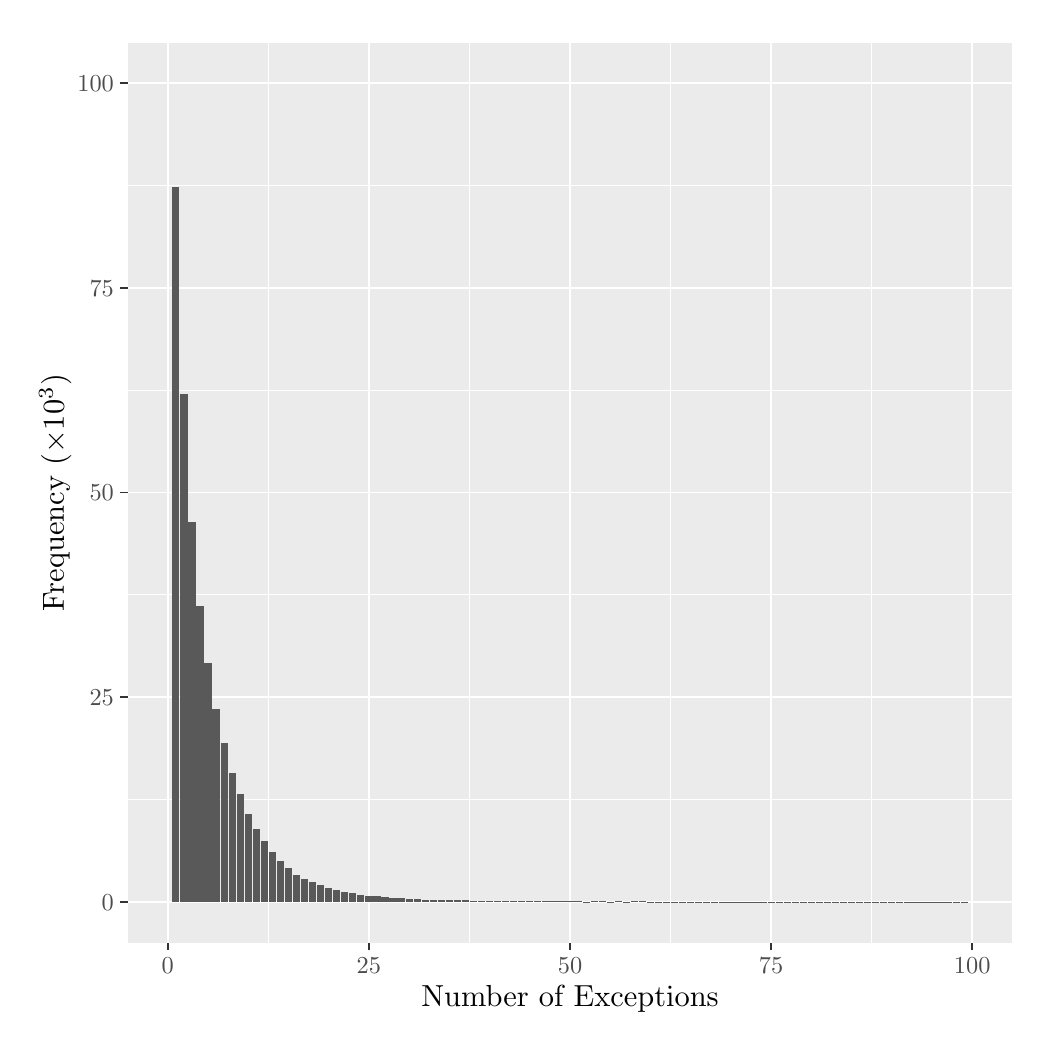
\begin{tikzpicture}[x=1pt,y=1pt]
\definecolor{fillColor}{RGB}{255,255,255}
\path[use as bounding box,fill=fillColor,fill opacity=0.00] (0,0) rectangle (361.35,361.35);
\begin{scope}
\path[clip] (  0.00,  0.00) rectangle (361.35,361.35);
\definecolor{drawColor}{RGB}{255,255,255}
\definecolor{fillColor}{RGB}{255,255,255}

\path[draw=drawColor,line width= 0.6pt,line join=round,line cap=round,fill=fillColor] (  0.00,  0.00) rectangle (361.35,361.35);
\end{scope}
\begin{scope}
\path[clip] ( 36.11, 30.69) rectangle (355.85,355.85);
\definecolor{fillColor}{gray}{0.92}

\path[fill=fillColor] ( 36.11, 30.69) rectangle (355.85,355.85);
\definecolor{drawColor}{RGB}{255,255,255}

\path[draw=drawColor,line width= 0.3pt,line join=round] ( 36.11, 82.45) --
	(355.85, 82.45);

\path[draw=drawColor,line width= 0.3pt,line join=round] ( 36.11,156.42) --
	(355.85,156.42);

\path[draw=drawColor,line width= 0.3pt,line join=round] ( 36.11,230.38) --
	(355.85,230.38);

\path[draw=drawColor,line width= 0.3pt,line join=round] ( 36.11,304.35) --
	(355.85,304.35);

\path[draw=drawColor,line width= 0.3pt,line join=round] ( 86.98, 30.69) --
	( 86.98,355.85);

\path[draw=drawColor,line width= 0.3pt,line join=round] (159.65, 30.69) --
	(159.65,355.85);

\path[draw=drawColor,line width= 0.3pt,line join=round] (232.31, 30.69) --
	(232.31,355.85);

\path[draw=drawColor,line width= 0.3pt,line join=round] (304.98, 30.69) --
	(304.98,355.85);

\path[draw=drawColor,line width= 0.6pt,line join=round] ( 36.11, 45.47) --
	(355.85, 45.47);

\path[draw=drawColor,line width= 0.6pt,line join=round] ( 36.11,119.43) --
	(355.85,119.43);

\path[draw=drawColor,line width= 0.6pt,line join=round] ( 36.11,193.40) --
	(355.85,193.40);

\path[draw=drawColor,line width= 0.6pt,line join=round] ( 36.11,267.37) --
	(355.85,267.37);

\path[draw=drawColor,line width= 0.6pt,line join=round] ( 36.11,341.34) --
	(355.85,341.34);

\path[draw=drawColor,line width= 0.6pt,line join=round] ( 50.64, 30.69) --
	( 50.64,355.85);

\path[draw=drawColor,line width= 0.6pt,line join=round] (123.31, 30.69) --
	(123.31,355.85);

\path[draw=drawColor,line width= 0.6pt,line join=round] (195.98, 30.69) --
	(195.98,355.85);

\path[draw=drawColor,line width= 0.6pt,line join=round] (268.65, 30.69) --
	(268.65,355.85);

\path[draw=drawColor,line width= 0.6pt,line join=round] (341.32, 30.69) --
	(341.32,355.85);
\definecolor{fillColor}{gray}{0.35}

\path[fill=fillColor] ( 52.24, 45.47) rectangle ( 54.86,303.76);

\path[fill=fillColor] ( 55.15, 45.47) rectangle ( 57.77,229.02);

\path[fill=fillColor] ( 58.06, 45.47) rectangle ( 60.67,182.55);

\path[fill=fillColor] ( 60.96, 45.47) rectangle ( 63.58,152.28);

\path[fill=fillColor] ( 63.87, 45.47) rectangle ( 66.49,131.71);

\path[fill=fillColor] ( 66.78, 45.47) rectangle ( 69.39,115.27);

\path[fill=fillColor] ( 69.68, 45.47) rectangle ( 72.30,103.03);

\path[fill=fillColor] ( 72.59, 45.47) rectangle ( 75.21, 92.15);

\path[fill=fillColor] ( 75.50, 45.47) rectangle ( 78.11, 84.47);

\path[fill=fillColor] ( 78.40, 45.47) rectangle ( 81.02, 77.36);

\path[fill=fillColor] ( 81.31, 45.47) rectangle ( 83.93, 71.87);

\path[fill=fillColor] ( 84.22, 45.47) rectangle ( 86.83, 67.43);

\path[fill=fillColor] ( 87.12, 45.47) rectangle ( 89.74, 63.64);

\path[fill=fillColor] ( 90.03, 45.47) rectangle ( 92.65, 60.19);

\path[fill=fillColor] ( 92.94, 45.47) rectangle ( 95.55, 57.70);

\path[fill=fillColor] ( 95.84, 45.47) rectangle ( 98.46, 55.08);

\path[fill=fillColor] ( 98.75, 45.47) rectangle (101.37, 53.84);

\path[fill=fillColor] (101.66, 45.47) rectangle (104.27, 52.65);

\path[fill=fillColor] (104.56, 45.47) rectangle (107.18, 51.51);

\path[fill=fillColor] (107.47, 45.47) rectangle (110.09, 50.42);

\path[fill=fillColor] (110.38, 45.47) rectangle (112.99, 49.62);

\path[fill=fillColor] (113.28, 45.47) rectangle (115.90, 48.95);

\path[fill=fillColor] (116.19, 45.47) rectangle (118.81, 48.54);

\path[fill=fillColor] (119.10, 45.47) rectangle (121.71, 48.05);

\path[fill=fillColor] (122.00, 45.47) rectangle (124.62, 47.58);

\path[fill=fillColor] (124.91, 45.47) rectangle (127.53, 47.40);

\path[fill=fillColor] (127.82, 45.47) rectangle (130.43, 47.26);

\path[fill=fillColor] (130.72, 45.47) rectangle (133.34, 46.87);

\path[fill=fillColor] (133.63, 45.47) rectangle (136.25, 46.79);

\path[fill=fillColor] (136.54, 45.47) rectangle (139.15, 46.48);

\path[fill=fillColor] (139.44, 45.47) rectangle (142.06, 46.53);

\path[fill=fillColor] (142.35, 45.47) rectangle (144.97, 46.31);

\path[fill=fillColor] (145.26, 45.47) rectangle (147.87, 46.29);

\path[fill=fillColor] (148.17, 45.47) rectangle (150.78, 46.20);

\path[fill=fillColor] (151.07, 45.47) rectangle (153.69, 46.11);

\path[fill=fillColor] (153.98, 45.47) rectangle (156.59, 45.98);

\path[fill=fillColor] (156.89, 45.47) rectangle (159.50, 46.01);

\path[fill=fillColor] (159.79, 45.47) rectangle (162.41, 45.94);

\path[fill=fillColor] (162.70, 45.47) rectangle (165.31, 45.80);

\path[fill=fillColor] (165.61, 45.47) rectangle (168.22, 45.91);

\path[fill=fillColor] (168.51, 45.47) rectangle (171.13, 45.81);

\path[fill=fillColor] (171.42, 45.47) rectangle (174.03, 45.73);

\path[fill=fillColor] (174.33, 45.47) rectangle (176.94, 45.84);

\path[fill=fillColor] (177.23, 45.47) rectangle (179.85, 45.73);

\path[fill=fillColor] (180.14, 45.47) rectangle (182.76, 45.74);

\path[fill=fillColor] (183.05, 45.47) rectangle (185.66, 45.74);

\path[fill=fillColor] (185.95, 45.47) rectangle (188.57, 45.67);

\path[fill=fillColor] (188.86, 45.47) rectangle (191.48, 45.69);

\path[fill=fillColor] (191.77, 45.47) rectangle (194.38, 45.65);

\path[fill=fillColor] (194.67, 45.47) rectangle (197.29, 45.68);

\path[fill=fillColor] (197.58, 45.47) rectangle (200.20, 45.71);

\path[fill=fillColor] (200.49, 45.47) rectangle (203.10, 45.59);

\path[fill=fillColor] (203.39, 45.47) rectangle (206.01, 45.66);

\path[fill=fillColor] (206.30, 45.47) rectangle (208.92, 45.63);

\path[fill=fillColor] (209.21, 45.47) rectangle (211.82, 45.59);

\path[fill=fillColor] (212.11, 45.47) rectangle (214.73, 45.60);

\path[fill=fillColor] (215.02, 45.47) rectangle (217.64, 45.58);

\path[fill=fillColor] (217.93, 45.47) rectangle (220.54, 45.62);

\path[fill=fillColor] (220.83, 45.47) rectangle (223.45, 45.60);

\path[fill=fillColor] (223.74, 45.47) rectangle (226.36, 45.55);

\path[fill=fillColor] (226.65, 45.47) rectangle (229.26, 45.57);

\path[fill=fillColor] (229.55, 45.47) rectangle (232.17, 45.55);

\path[fill=fillColor] (232.46, 45.47) rectangle (235.08, 45.56);

\path[fill=fillColor] (235.37, 45.47) rectangle (237.98, 45.56);

\path[fill=fillColor] (238.27, 45.47) rectangle (240.89, 45.55);

\path[fill=fillColor] (241.18, 45.47) rectangle (243.80, 45.52);

\path[fill=fillColor] (244.09, 45.47) rectangle (246.70, 45.53);

\path[fill=fillColor] (246.99, 45.47) rectangle (249.61, 45.57);

\path[fill=fillColor] (249.90, 45.47) rectangle (252.52, 45.54);

\path[fill=fillColor] (252.81, 45.47) rectangle (255.42, 45.54);

\path[fill=fillColor] (255.71, 45.47) rectangle (258.33, 45.53);

\path[fill=fillColor] (258.62, 45.47) rectangle (261.24, 45.51);

\path[fill=fillColor] (261.53, 45.47) rectangle (264.14, 45.53);

\path[fill=fillColor] (264.43, 45.47) rectangle (267.05, 45.50);

\path[fill=fillColor] (267.34, 45.47) rectangle (269.96, 45.52);

\path[fill=fillColor] (270.25, 45.47) rectangle (272.86, 45.53);

\path[fill=fillColor] (273.15, 45.47) rectangle (275.77, 45.53);

\path[fill=fillColor] (276.06, 45.47) rectangle (278.68, 45.51);

\path[fill=fillColor] (278.97, 45.47) rectangle (281.58, 45.53);

\path[fill=fillColor] (281.87, 45.47) rectangle (284.49, 45.53);

\path[fill=fillColor] (284.78, 45.47) rectangle (287.40, 45.50);

\path[fill=fillColor] (287.69, 45.47) rectangle (290.30, 45.50);

\path[fill=fillColor] (290.59, 45.47) rectangle (293.21, 45.49);

\path[fill=fillColor] (293.50, 45.47) rectangle (296.12, 45.51);

\path[fill=fillColor] (296.41, 45.47) rectangle (299.02, 45.50);

\path[fill=fillColor] (299.31, 45.47) rectangle (301.93, 45.53);

\path[fill=fillColor] (302.22, 45.47) rectangle (304.84, 45.51);

\path[fill=fillColor] (305.13, 45.47) rectangle (307.74, 45.51);

\path[fill=fillColor] (308.03, 45.47) rectangle (310.65, 45.51);

\path[fill=fillColor] (310.94, 45.47) rectangle (313.56, 45.50);

\path[fill=fillColor] (313.85, 45.47) rectangle (316.46, 45.50);

\path[fill=fillColor] (316.75, 45.47) rectangle (319.37, 45.53);

\path[fill=fillColor] (319.66, 45.47) rectangle (322.28, 45.50);

\path[fill=fillColor] (322.57, 45.47) rectangle (325.18, 45.50);

\path[fill=fillColor] (325.47, 45.47) rectangle (328.09, 45.51);

\path[fill=fillColor] (328.38, 45.47) rectangle (331.00, 45.50);

\path[fill=fillColor] (331.29, 45.47) rectangle (333.90, 45.51);

\path[fill=fillColor] (334.19, 45.47) rectangle (336.81, 45.50);

\path[fill=fillColor] (337.10, 45.47) rectangle (339.72, 45.49);
\end{scope}
\begin{scope}
\path[clip] (  0.00,  0.00) rectangle (361.35,361.35);
\definecolor{drawColor}{gray}{0.30}

\node[text=drawColor,anchor=base east,inner sep=0pt, outer sep=0pt, scale=  0.88] at ( 31.16, 42.44) {0};

\node[text=drawColor,anchor=base east,inner sep=0pt, outer sep=0pt, scale=  0.88] at ( 31.16,116.40) {25};

\node[text=drawColor,anchor=base east,inner sep=0pt, outer sep=0pt, scale=  0.88] at ( 31.16,190.37) {50};

\node[text=drawColor,anchor=base east,inner sep=0pt, outer sep=0pt, scale=  0.88] at ( 31.16,264.34) {75};

\node[text=drawColor,anchor=base east,inner sep=0pt, outer sep=0pt, scale=  0.88] at ( 31.16,338.31) {100};
\end{scope}
\begin{scope}
\path[clip] (  0.00,  0.00) rectangle (361.35,361.35);
\definecolor{drawColor}{gray}{0.20}

\path[draw=drawColor,line width= 0.6pt,line join=round] ( 33.36, 45.47) --
	( 36.11, 45.47);

\path[draw=drawColor,line width= 0.6pt,line join=round] ( 33.36,119.43) --
	( 36.11,119.43);

\path[draw=drawColor,line width= 0.6pt,line join=round] ( 33.36,193.40) --
	( 36.11,193.40);

\path[draw=drawColor,line width= 0.6pt,line join=round] ( 33.36,267.37) --
	( 36.11,267.37);

\path[draw=drawColor,line width= 0.6pt,line join=round] ( 33.36,341.34) --
	( 36.11,341.34);
\end{scope}
\begin{scope}
\path[clip] (  0.00,  0.00) rectangle (361.35,361.35);
\definecolor{drawColor}{gray}{0.20}

\path[draw=drawColor,line width= 0.6pt,line join=round] ( 50.64, 27.94) --
	( 50.64, 30.69);

\path[draw=drawColor,line width= 0.6pt,line join=round] (123.31, 27.94) --
	(123.31, 30.69);

\path[draw=drawColor,line width= 0.6pt,line join=round] (195.98, 27.94) --
	(195.98, 30.69);

\path[draw=drawColor,line width= 0.6pt,line join=round] (268.65, 27.94) --
	(268.65, 30.69);

\path[draw=drawColor,line width= 0.6pt,line join=round] (341.32, 27.94) --
	(341.32, 30.69);
\end{scope}
\begin{scope}
\path[clip] (  0.00,  0.00) rectangle (361.35,361.35);
\definecolor{drawColor}{gray}{0.30}

\node[text=drawColor,anchor=base,inner sep=0pt, outer sep=0pt, scale=  0.88] at ( 50.64, 19.68) {0};

\node[text=drawColor,anchor=base,inner sep=0pt, outer sep=0pt, scale=  0.88] at (123.31, 19.68) {25};

\node[text=drawColor,anchor=base,inner sep=0pt, outer sep=0pt, scale=  0.88] at (195.98, 19.68) {50};

\node[text=drawColor,anchor=base,inner sep=0pt, outer sep=0pt, scale=  0.88] at (268.65, 19.68) {75};

\node[text=drawColor,anchor=base,inner sep=0pt, outer sep=0pt, scale=  0.88] at (341.32, 19.68) {100};
\end{scope}
\begin{scope}
\path[clip] (  0.00,  0.00) rectangle (361.35,361.35);
\definecolor{drawColor}{RGB}{0,0,0}

\node[text=drawColor,anchor=base,inner sep=0pt, outer sep=0pt, scale=  1.10] at (195.98,  7.64) {Number of Exceptions};
\end{scope}
\begin{scope}
\path[clip] (  0.00,  0.00) rectangle (361.35,361.35);
\definecolor{drawColor}{RGB}{0,0,0}

\node[text=drawColor,rotate= 90.00,anchor=base,inner sep=0pt, outer sep=0pt, scale=  1.10] at ( 13.08,193.27) {Frequency ($\times 10^3$)};
\end{scope}
\end{tikzpicture}

	\caption[Histogram of the number of exceptions per read.]{\label{fig:nex-hist}Histogram of the number of exceptions per read up to 100 which appears to nicely follow an exponential distribution. Values after 100 occur highly infrequently -- there are only 546 out of \num{500000} reads with more than 100 exceptions.}
\end{figure}


The exceptions range from 256 to 2317 as expected but 99\% of the exceptions do not go higher than 481. The mean and mode are $\sim$277 and 256 respectively. Refer to Table \ref{tab:ex}. The histogram of exceptions is shown in Figure \ref{fig:ex-hist}. Notably, the frequency of even-numbered exceptions is much greater than adjacent odd-numbered exceptions from 256 up to $\sim$330. This is due to large positive deltas occuring more frequently than large negative deltas as previously discussed in Section \ref{subsec:stripe}.

\begin{figure}
	\centering
% Created by tikzDevice version 0.12.3.1 on 2022-10-11 17:28:28
% !TEX encoding = UTF-8 Unicode
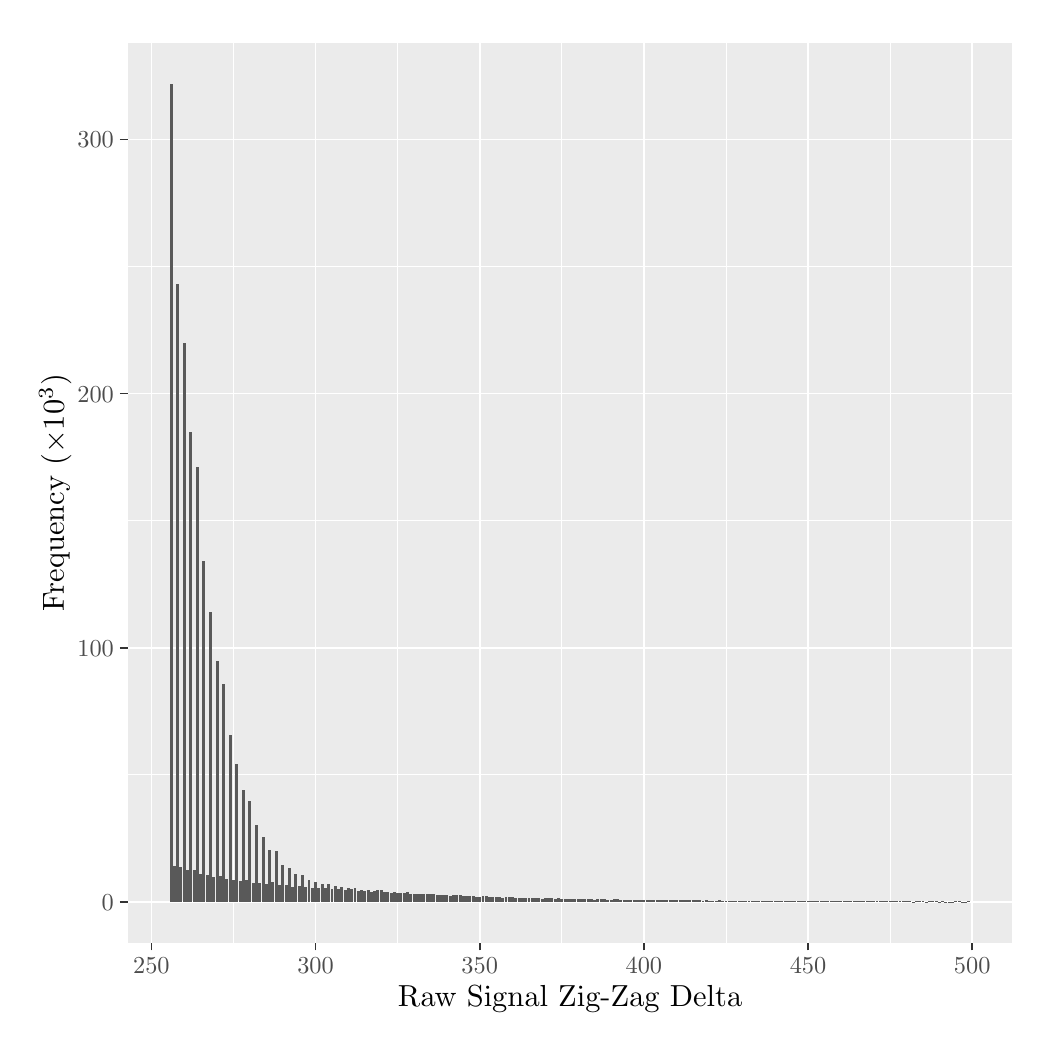
\begin{tikzpicture}[x=1pt,y=1pt]
\definecolor{fillColor}{RGB}{255,255,255}
\path[use as bounding box,fill=fillColor,fill opacity=0.00] (0,0) rectangle (361.35,361.35);
\begin{scope}
\path[clip] (  0.00,  0.00) rectangle (361.35,361.35);
\definecolor{drawColor}{RGB}{255,255,255}
\definecolor{fillColor}{RGB}{255,255,255}

\path[draw=drawColor,line width= 0.6pt,line join=round,line cap=round,fill=fillColor] (  0.00,  0.00) rectangle (361.35,361.35);
\end{scope}
\begin{scope}
\path[clip] ( 36.11, 30.69) rectangle (355.85,355.85);
\definecolor{fillColor}{gray}{0.92}

\path[fill=fillColor] ( 36.11, 30.69) rectangle (355.85,355.85);
\definecolor{drawColor}{RGB}{255,255,255}

\path[draw=drawColor,line width= 0.3pt,line join=round] ( 36.11, 91.37) --
	(355.85, 91.37);

\path[draw=drawColor,line width= 0.3pt,line join=round] ( 36.11,183.19) --
	(355.85,183.19);

\path[draw=drawColor,line width= 0.3pt,line join=round] ( 36.11,275.01) --
	(355.85,275.01);

\path[draw=drawColor,line width= 0.3pt,line join=round] ( 74.37, 30.69) --
	( 74.37,355.85);

\path[draw=drawColor,line width= 0.3pt,line join=round] (133.69, 30.69) --
	(133.69,355.85);

\path[draw=drawColor,line width= 0.3pt,line join=round] (193.01, 30.69) --
	(193.01,355.85);

\path[draw=drawColor,line width= 0.3pt,line join=round] (252.34, 30.69) --
	(252.34,355.85);

\path[draw=drawColor,line width= 0.3pt,line join=round] (311.66, 30.69) --
	(311.66,355.85);

\path[draw=drawColor,line width= 0.6pt,line join=round] ( 36.11, 45.47) --
	(355.85, 45.47);

\path[draw=drawColor,line width= 0.6pt,line join=round] ( 36.11,137.28) --
	(355.85,137.28);

\path[draw=drawColor,line width= 0.6pt,line join=round] ( 36.11,229.10) --
	(355.85,229.10);

\path[draw=drawColor,line width= 0.6pt,line join=round] ( 36.11,320.91) --
	(355.85,320.91);

\path[draw=drawColor,line width= 0.6pt,line join=round] ( 44.71, 30.69) --
	( 44.71,355.85);

\path[draw=drawColor,line width= 0.6pt,line join=round] (104.03, 30.69) --
	(104.03,355.85);

\path[draw=drawColor,line width= 0.6pt,line join=round] (163.35, 30.69) --
	(163.35,355.85);

\path[draw=drawColor,line width= 0.6pt,line join=round] (222.67, 30.69) --
	(222.67,355.85);

\path[draw=drawColor,line width= 0.6pt,line join=round] (282.00, 30.69) --
	(282.00,355.85);

\path[draw=drawColor,line width= 0.6pt,line join=round] (341.32, 30.69) --
	(341.32,355.85);
\definecolor{fillColor}{gray}{0.35}

\path[fill=fillColor] ( 51.30, 45.47) rectangle ( 52.37,341.07);

\path[fill=fillColor] ( 52.48, 45.47) rectangle ( 53.55, 58.32);

\path[fill=fillColor] ( 53.67, 45.47) rectangle ( 54.74,268.74);

\path[fill=fillColor] ( 54.86, 45.47) rectangle ( 55.92, 58.08);

\path[fill=fillColor] ( 56.04, 45.47) rectangle ( 57.11,247.36);

\path[fill=fillColor] ( 57.23, 45.47) rectangle ( 58.30, 56.94);

\path[fill=fillColor] ( 58.42, 45.47) rectangle ( 59.48,215.13);

\path[fill=fillColor] ( 59.60, 45.47) rectangle ( 60.67, 57.07);

\path[fill=fillColor] ( 60.79, 45.47) rectangle ( 61.86,202.50);

\path[fill=fillColor] ( 61.98, 45.47) rectangle ( 63.04, 55.42);

\path[fill=fillColor] ( 63.16, 45.47) rectangle ( 64.23,168.69);

\path[fill=fillColor] ( 64.35, 45.47) rectangle ( 65.42, 55.18);

\path[fill=fillColor] ( 65.53, 45.47) rectangle ( 66.60,150.14);

\path[fill=fillColor] ( 66.72, 45.47) rectangle ( 67.79, 54.37);

\path[fill=fillColor] ( 67.91, 45.47) rectangle ( 68.97,132.62);

\path[fill=fillColor] ( 69.09, 45.47) rectangle ( 70.16, 54.86);

\path[fill=fillColor] ( 70.28, 45.47) rectangle ( 71.35,124.30);

\path[fill=fillColor] ( 71.47, 45.47) rectangle ( 72.53, 53.65);

\path[fill=fillColor] ( 72.65, 45.47) rectangle ( 73.72,105.80);

\path[fill=fillColor] ( 73.84, 45.47) rectangle ( 74.91, 53.53);

\path[fill=fillColor] ( 75.03, 45.47) rectangle ( 76.09, 95.30);

\path[fill=fillColor] ( 76.21, 45.47) rectangle ( 77.28, 53.03);

\path[fill=fillColor] ( 77.40, 45.47) rectangle ( 78.47, 85.80);

\path[fill=fillColor] ( 78.58, 45.47) rectangle ( 79.65, 53.38);

\path[fill=fillColor] ( 79.77, 45.47) rectangle ( 80.84, 81.94);

\path[fill=fillColor] ( 80.96, 45.47) rectangle ( 82.03, 52.23);

\path[fill=fillColor] ( 82.14, 45.47) rectangle ( 83.21, 73.06);

\path[fill=fillColor] ( 83.33, 45.47) rectangle ( 84.40, 52.19);

\path[fill=fillColor] ( 84.52, 45.47) rectangle ( 85.58, 68.84);

\path[fill=fillColor] ( 85.70, 45.47) rectangle ( 86.77, 51.88);

\path[fill=fillColor] ( 86.89, 45.47) rectangle ( 87.96, 64.21);

\path[fill=fillColor] ( 88.08, 45.47) rectangle ( 89.14, 52.55);

\path[fill=fillColor] ( 89.26, 45.47) rectangle ( 90.33, 63.73);

\path[fill=fillColor] ( 90.45, 45.47) rectangle ( 91.52, 51.52);

\path[fill=fillColor] ( 91.64, 45.47) rectangle ( 92.70, 58.82);

\path[fill=fillColor] ( 92.82, 45.47) rectangle ( 93.89, 51.40);

\path[fill=fillColor] ( 94.01, 45.47) rectangle ( 95.08, 57.60);

\path[fill=fillColor] ( 95.19, 45.47) rectangle ( 96.26, 51.00);

\path[fill=fillColor] ( 96.38, 45.47) rectangle ( 97.45, 55.59);

\path[fill=fillColor] ( 97.57, 45.47) rectangle ( 98.64, 51.22);

\path[fill=fillColor] ( 98.75, 45.47) rectangle ( 99.82, 55.06);

\path[fill=fillColor] ( 99.94, 45.47) rectangle (101.01, 50.82);

\path[fill=fillColor] (101.13, 45.47) rectangle (102.19, 53.45);

\path[fill=fillColor] (102.31, 45.47) rectangle (103.38, 50.61);

\path[fill=fillColor] (103.50, 45.47) rectangle (104.57, 52.63);

\path[fill=fillColor] (104.69, 45.47) rectangle (105.75, 50.39);

\path[fill=fillColor] (105.87, 45.47) rectangle (106.94, 52.08);

\path[fill=fillColor] (107.06, 45.47) rectangle (108.13, 50.65);

\path[fill=fillColor] (108.25, 45.47) rectangle (109.31, 52.00);

\path[fill=fillColor] (109.43, 45.47) rectangle (110.50, 50.26);

\path[fill=fillColor] (110.62, 45.47) rectangle (111.69, 51.13);

\path[fill=fillColor] (111.80, 45.47) rectangle (112.87, 50.05);

\path[fill=fillColor] (112.99, 45.47) rectangle (114.06, 50.72);

\path[fill=fillColor] (114.18, 45.47) rectangle (115.25, 49.84);

\path[fill=fillColor] (115.36, 45.47) rectangle (116.43, 50.38);

\path[fill=fillColor] (116.55, 45.47) rectangle (117.62, 50.03);

\path[fill=fillColor] (117.74, 45.47) rectangle (118.80, 50.45);

\path[fill=fillColor] (118.92, 45.47) rectangle (119.99, 49.53);

\path[fill=fillColor] (120.11, 45.47) rectangle (121.18, 49.83);

\path[fill=fillColor] (121.30, 45.47) rectangle (122.36, 49.34);

\path[fill=fillColor] (122.48, 45.47) rectangle (123.55, 49.74);

\path[fill=fillColor] (123.67, 45.47) rectangle (124.74, 49.20);

\path[fill=fillColor] (124.86, 45.47) rectangle (125.92, 49.39);

\path[fill=fillColor] (126.04, 45.47) rectangle (127.11, 49.63);

\path[fill=fillColor] (127.23, 45.47) rectangle (128.30, 49.72);

\path[fill=fillColor] (128.41, 45.47) rectangle (129.48, 48.89);

\path[fill=fillColor] (129.60, 45.47) rectangle (130.67, 49.02);

\path[fill=fillColor] (130.79, 45.47) rectangle (131.85, 48.70);

\path[fill=fillColor] (131.97, 45.47) rectangle (133.04, 49.02);

\path[fill=fillColor] (133.16, 45.47) rectangle (134.23, 48.56);

\path[fill=fillColor] (134.35, 45.47) rectangle (135.41, 48.63);

\path[fill=fillColor] (135.53, 45.47) rectangle (136.60, 48.78);

\path[fill=fillColor] (136.72, 45.47) rectangle (137.79, 48.94);

\path[fill=fillColor] (137.91, 45.47) rectangle (138.97, 48.45);

\path[fill=fillColor] (139.09, 45.47) rectangle (140.16, 48.45);

\path[fill=fillColor] (140.28, 45.47) rectangle (141.35, 48.29);

\path[fill=fillColor] (141.46, 45.47) rectangle (142.53, 48.26);

\path[fill=fillColor] (142.65, 45.47) rectangle (143.72, 48.14);

\path[fill=fillColor] (143.84, 45.47) rectangle (144.91, 48.13);

\path[fill=fillColor] (145.02, 45.47) rectangle (146.09, 48.21);

\path[fill=fillColor] (146.21, 45.47) rectangle (147.28, 48.16);

\path[fill=fillColor] (147.40, 45.47) rectangle (148.46, 47.87);

\path[fill=fillColor] (148.58, 45.47) rectangle (149.65, 48.02);

\path[fill=fillColor] (149.77, 45.47) rectangle (150.84, 47.77);

\path[fill=fillColor] (150.96, 45.47) rectangle (152.02, 47.92);

\path[fill=fillColor] (152.14, 45.47) rectangle (153.21, 47.64);

\path[fill=fillColor] (153.33, 45.47) rectangle (154.40, 47.79);

\path[fill=fillColor] (154.52, 45.47) rectangle (155.58, 47.79);

\path[fill=fillColor] (155.70, 45.47) rectangle (156.77, 47.87);

\path[fill=fillColor] (156.89, 45.47) rectangle (157.96, 47.41);

\path[fill=fillColor] (158.07, 45.47) rectangle (159.14, 47.60);

\path[fill=fillColor] (159.26, 45.47) rectangle (160.33, 47.45);

\path[fill=fillColor] (160.45, 45.47) rectangle (161.52, 47.53);

\path[fill=fillColor] (161.63, 45.47) rectangle (162.70, 47.28);

\path[fill=fillColor] (162.82, 45.47) rectangle (163.89, 47.36);

\path[fill=fillColor] (164.01, 45.47) rectangle (165.07, 47.44);

\path[fill=fillColor] (165.19, 45.47) rectangle (166.26, 47.53);

\path[fill=fillColor] (166.38, 45.47) rectangle (167.45, 47.16);

\path[fill=fillColor] (167.57, 45.47) rectangle (168.63, 47.28);

\path[fill=fillColor] (168.75, 45.47) rectangle (169.82, 47.08);

\path[fill=fillColor] (169.94, 45.47) rectangle (171.01, 47.23);

\path[fill=fillColor] (171.13, 45.47) rectangle (172.19, 47.01);

\path[fill=fillColor] (172.31, 45.47) rectangle (173.38, 47.12);

\path[fill=fillColor] (173.50, 45.47) rectangle (174.57, 47.07);

\path[fill=fillColor] (174.68, 45.47) rectangle (175.75, 47.10);

\path[fill=fillColor] (175.87, 45.47) rectangle (176.94, 46.90);

\path[fill=fillColor] (177.06, 45.47) rectangle (178.13, 46.95);

\path[fill=fillColor] (178.24, 45.47) rectangle (179.31, 46.84);

\path[fill=fillColor] (179.43, 45.47) rectangle (180.50, 46.93);

\path[fill=fillColor] (180.62, 45.47) rectangle (181.68, 46.77);

\path[fill=fillColor] (181.80, 45.47) rectangle (182.87, 46.83);

\path[fill=fillColor] (182.99, 45.47) rectangle (184.06, 46.79);

\path[fill=fillColor] (184.18, 45.47) rectangle (185.24, 46.87);

\path[fill=fillColor] (185.36, 45.47) rectangle (186.43, 46.66);

\path[fill=fillColor] (186.55, 45.47) rectangle (187.62, 46.70);

\path[fill=fillColor] (187.74, 45.47) rectangle (188.80, 46.69);

\path[fill=fillColor] (188.92, 45.47) rectangle (189.99, 46.71);

\path[fill=fillColor] (190.11, 45.47) rectangle (191.18, 46.63);

\path[fill=fillColor] (191.29, 45.47) rectangle (192.36, 46.68);

\path[fill=fillColor] (192.48, 45.47) rectangle (193.55, 46.65);

\path[fill=fillColor] (193.67, 45.47) rectangle (194.73, 46.63);

\path[fill=fillColor] (194.85, 45.47) rectangle (195.92, 46.46);

\path[fill=fillColor] (196.04, 45.47) rectangle (197.11, 46.51);

\path[fill=fillColor] (197.23, 45.47) rectangle (198.29, 46.47);

\path[fill=fillColor] (198.41, 45.47) rectangle (199.48, 46.48);

\path[fill=fillColor] (199.60, 45.47) rectangle (200.67, 46.41);

\path[fill=fillColor] (200.79, 45.47) rectangle (201.85, 46.41);

\path[fill=fillColor] (201.97, 45.47) rectangle (203.04, 46.48);

\path[fill=fillColor] (203.16, 45.47) rectangle (204.23, 46.55);

\path[fill=fillColor] (204.34, 45.47) rectangle (205.41, 46.29);

\path[fill=fillColor] (205.53, 45.47) rectangle (206.60, 46.39);

\path[fill=fillColor] (206.72, 45.47) rectangle (207.79, 46.33);

\path[fill=fillColor] (207.90, 45.47) rectangle (208.97, 46.36);

\path[fill=fillColor] (209.09, 45.47) rectangle (210.16, 46.31);

\path[fill=fillColor] (210.28, 45.47) rectangle (211.34, 46.30);

\path[fill=fillColor] (211.46, 45.47) rectangle (212.53, 46.36);

\path[fill=fillColor] (212.65, 45.47) rectangle (213.72, 46.35);

\path[fill=fillColor] (213.84, 45.47) rectangle (214.90, 46.19);

\path[fill=fillColor] (215.02, 45.47) rectangle (216.09, 46.23);

\path[fill=fillColor] (216.21, 45.47) rectangle (217.28, 46.21);

\path[fill=fillColor] (217.40, 45.47) rectangle (218.46, 46.19);

\path[fill=fillColor] (218.58, 45.47) rectangle (219.65, 46.21);

\path[fill=fillColor] (219.77, 45.47) rectangle (220.84, 46.18);

\path[fill=fillColor] (220.95, 45.47) rectangle (222.02, 46.17);

\path[fill=fillColor] (222.14, 45.47) rectangle (223.21, 46.19);

\path[fill=fillColor] (223.33, 45.47) rectangle (224.40, 46.18);

\path[fill=fillColor] (224.51, 45.47) rectangle (225.58, 46.12);

\path[fill=fillColor] (225.70, 45.47) rectangle (226.77, 46.08);

\path[fill=fillColor] (226.89, 45.47) rectangle (227.95, 46.10);

\path[fill=fillColor] (228.07, 45.47) rectangle (229.14, 46.09);

\path[fill=fillColor] (229.26, 45.47) rectangle (230.33, 46.07);

\path[fill=fillColor] (230.45, 45.47) rectangle (231.51, 46.13);

\path[fill=fillColor] (231.63, 45.47) rectangle (232.70, 46.04);

\path[fill=fillColor] (232.82, 45.47) rectangle (233.89, 46.04);

\path[fill=fillColor] (234.01, 45.47) rectangle (235.07, 45.98);

\path[fill=fillColor] (235.19, 45.47) rectangle (236.26, 46.03);

\path[fill=fillColor] (236.38, 45.47) rectangle (237.45, 45.97);

\path[fill=fillColor] (237.56, 45.47) rectangle (238.63, 46.03);

\path[fill=fillColor] (238.75, 45.47) rectangle (239.82, 45.99);

\path[fill=fillColor] (239.94, 45.47) rectangle (241.01, 46.09);

\path[fill=fillColor] (241.12, 45.47) rectangle (242.19, 46.03);

\path[fill=fillColor] (242.31, 45.47) rectangle (243.38, 45.97);

\path[fill=fillColor] (243.50, 45.47) rectangle (244.56, 45.91);

\path[fill=fillColor] (244.68, 45.47) rectangle (245.75, 46.00);

\path[fill=fillColor] (245.87, 45.47) rectangle (246.94, 45.90);

\path[fill=fillColor] (247.06, 45.47) rectangle (248.12, 45.93);

\path[fill=fillColor] (248.24, 45.47) rectangle (249.31, 45.86);

\path[fill=fillColor] (249.43, 45.47) rectangle (250.50, 45.96);

\path[fill=fillColor] (250.61, 45.47) rectangle (251.68, 45.90);

\path[fill=fillColor] (251.80, 45.47) rectangle (252.87, 45.95);

\path[fill=fillColor] (252.99, 45.47) rectangle (254.06, 45.87);

\path[fill=fillColor] (254.17, 45.47) rectangle (255.24, 45.86);

\path[fill=fillColor] (255.36, 45.47) rectangle (256.43, 45.84);

\path[fill=fillColor] (256.55, 45.47) rectangle (257.61, 45.86);

\path[fill=fillColor] (257.73, 45.47) rectangle (258.80, 45.85);

\path[fill=fillColor] (258.92, 45.47) rectangle (259.99, 45.89);

\path[fill=fillColor] (260.11, 45.47) rectangle (261.17, 45.83);

\path[fill=fillColor] (261.29, 45.47) rectangle (262.36, 45.86);

\path[fill=fillColor] (262.48, 45.47) rectangle (263.55, 45.80);

\path[fill=fillColor] (263.67, 45.47) rectangle (264.73, 45.84);

\path[fill=fillColor] (264.85, 45.47) rectangle (265.92, 45.78);

\path[fill=fillColor] (266.04, 45.47) rectangle (267.11, 45.84);

\path[fill=fillColor] (267.22, 45.47) rectangle (268.29, 45.77);

\path[fill=fillColor] (268.41, 45.47) rectangle (269.48, 45.82);

\path[fill=fillColor] (269.60, 45.47) rectangle (270.67, 45.79);

\path[fill=fillColor] (270.78, 45.47) rectangle (271.85, 45.77);

\path[fill=fillColor] (271.97, 45.47) rectangle (273.04, 45.76);

\path[fill=fillColor] (273.16, 45.47) rectangle (274.22, 45.76);

\path[fill=fillColor] (274.34, 45.47) rectangle (275.41, 45.75);

\path[fill=fillColor] (275.53, 45.47) rectangle (276.60, 45.75);

\path[fill=fillColor] (276.72, 45.47) rectangle (277.78, 45.70);

\path[fill=fillColor] (277.90, 45.47) rectangle (278.97, 45.74);

\path[fill=fillColor] (279.09, 45.47) rectangle (280.16, 45.76);

\path[fill=fillColor] (280.28, 45.47) rectangle (281.34, 45.71);

\path[fill=fillColor] (281.46, 45.47) rectangle (282.53, 45.70);

\path[fill=fillColor] (282.65, 45.47) rectangle (283.72, 45.71);

\path[fill=fillColor] (283.83, 45.47) rectangle (284.90, 45.74);

\path[fill=fillColor] (285.02, 45.47) rectangle (286.09, 45.70);

\path[fill=fillColor] (286.21, 45.47) rectangle (287.28, 45.70);

\path[fill=fillColor] (287.39, 45.47) rectangle (288.46, 45.72);

\path[fill=fillColor] (288.58, 45.47) rectangle (289.65, 45.68);

\path[fill=fillColor] (289.77, 45.47) rectangle (290.83, 45.70);

\path[fill=fillColor] (290.95, 45.47) rectangle (292.02, 45.69);

\path[fill=fillColor] (292.14, 45.47) rectangle (293.21, 45.67);

\path[fill=fillColor] (293.33, 45.47) rectangle (294.39, 45.67);

\path[fill=fillColor] (294.51, 45.47) rectangle (295.58, 45.68);

\path[fill=fillColor] (295.70, 45.47) rectangle (296.77, 45.64);

\path[fill=fillColor] (296.89, 45.47) rectangle (297.95, 45.70);

\path[fill=fillColor] (298.07, 45.47) rectangle (299.14, 45.68);

\path[fill=fillColor] (299.26, 45.47) rectangle (300.33, 45.66);

\path[fill=fillColor] (300.44, 45.47) rectangle (301.51, 45.66);

\path[fill=fillColor] (301.63, 45.47) rectangle (302.70, 45.67);

\path[fill=fillColor] (302.82, 45.47) rectangle (303.89, 45.65);

\path[fill=fillColor] (304.00, 45.47) rectangle (305.07, 45.62);

\path[fill=fillColor] (305.19, 45.47) rectangle (306.26, 45.63);

\path[fill=fillColor] (306.38, 45.47) rectangle (307.44, 45.67);

\path[fill=fillColor] (307.56, 45.47) rectangle (308.63, 45.64);

\path[fill=fillColor] (308.75, 45.47) rectangle (309.82, 45.63);

\path[fill=fillColor] (309.94, 45.47) rectangle (311.00, 45.63);

\path[fill=fillColor] (311.12, 45.47) rectangle (312.19, 45.65);

\path[fill=fillColor] (312.31, 45.47) rectangle (313.38, 45.63);

\path[fill=fillColor] (313.49, 45.47) rectangle (314.56, 45.61);

\path[fill=fillColor] (314.68, 45.47) rectangle (315.75, 45.60);

\path[fill=fillColor] (315.87, 45.47) rectangle (316.94, 45.65);

\path[fill=fillColor] (317.05, 45.47) rectangle (318.12, 45.61);

\path[fill=fillColor] (318.24, 45.47) rectangle (319.31, 45.64);

\path[fill=fillColor] (319.43, 45.47) rectangle (320.49, 45.59);

\path[fill=fillColor] (320.61, 45.47) rectangle (321.68, 45.62);

\path[fill=fillColor] (321.80, 45.47) rectangle (322.87, 45.60);

\path[fill=fillColor] (322.99, 45.47) rectangle (324.05, 45.63);

\path[fill=fillColor] (324.17, 45.47) rectangle (325.24, 45.59);

\path[fill=fillColor] (325.36, 45.47) rectangle (326.43, 45.63);

\path[fill=fillColor] (326.55, 45.47) rectangle (327.61, 45.61);

\path[fill=fillColor] (327.73, 45.47) rectangle (328.80, 45.60);

\path[fill=fillColor] (328.92, 45.47) rectangle (329.99, 45.59);

\path[fill=fillColor] (330.10, 45.47) rectangle (331.17, 45.61);

\path[fill=fillColor] (331.29, 45.47) rectangle (332.36, 45.58);

\path[fill=fillColor] (332.48, 45.47) rectangle (333.55, 45.59);

\path[fill=fillColor] (333.66, 45.47) rectangle (334.73, 45.57);

\path[fill=fillColor] (334.85, 45.47) rectangle (335.92, 45.61);

\path[fill=fillColor] (336.04, 45.47) rectangle (337.10, 45.60);

\path[fill=fillColor] (337.22, 45.47) rectangle (338.29, 45.57);

\path[fill=fillColor] (338.41, 45.47) rectangle (339.48, 45.57);

\path[fill=fillColor] (339.60, 45.47) rectangle (340.66, 45.60);
\end{scope}
\begin{scope}
\path[clip] (  0.00,  0.00) rectangle (361.35,361.35);
\definecolor{drawColor}{gray}{0.30}

\node[text=drawColor,anchor=base east,inner sep=0pt, outer sep=0pt, scale=  0.88] at ( 31.16, 42.44) {0};

\node[text=drawColor,anchor=base east,inner sep=0pt, outer sep=0pt, scale=  0.88] at ( 31.16,134.25) {100};

\node[text=drawColor,anchor=base east,inner sep=0pt, outer sep=0pt, scale=  0.88] at ( 31.16,226.07) {200};

\node[text=drawColor,anchor=base east,inner sep=0pt, outer sep=0pt, scale=  0.88] at ( 31.16,317.88) {300};
\end{scope}
\begin{scope}
\path[clip] (  0.00,  0.00) rectangle (361.35,361.35);
\definecolor{drawColor}{gray}{0.20}

\path[draw=drawColor,line width= 0.6pt,line join=round] ( 33.36, 45.47) --
	( 36.11, 45.47);

\path[draw=drawColor,line width= 0.6pt,line join=round] ( 33.36,137.28) --
	( 36.11,137.28);

\path[draw=drawColor,line width= 0.6pt,line join=round] ( 33.36,229.10) --
	( 36.11,229.10);

\path[draw=drawColor,line width= 0.6pt,line join=round] ( 33.36,320.91) --
	( 36.11,320.91);
\end{scope}
\begin{scope}
\path[clip] (  0.00,  0.00) rectangle (361.35,361.35);
\definecolor{drawColor}{gray}{0.20}

\path[draw=drawColor,line width= 0.6pt,line join=round] ( 44.71, 27.94) --
	( 44.71, 30.69);

\path[draw=drawColor,line width= 0.6pt,line join=round] (104.03, 27.94) --
	(104.03, 30.69);

\path[draw=drawColor,line width= 0.6pt,line join=round] (163.35, 27.94) --
	(163.35, 30.69);

\path[draw=drawColor,line width= 0.6pt,line join=round] (222.67, 27.94) --
	(222.67, 30.69);

\path[draw=drawColor,line width= 0.6pt,line join=round] (282.00, 27.94) --
	(282.00, 30.69);

\path[draw=drawColor,line width= 0.6pt,line join=round] (341.32, 27.94) --
	(341.32, 30.69);
\end{scope}
\begin{scope}
\path[clip] (  0.00,  0.00) rectangle (361.35,361.35);
\definecolor{drawColor}{gray}{0.30}

\node[text=drawColor,anchor=base,inner sep=0pt, outer sep=0pt, scale=  0.88] at ( 44.71, 19.68) {250};

\node[text=drawColor,anchor=base,inner sep=0pt, outer sep=0pt, scale=  0.88] at (104.03, 19.68) {300};

\node[text=drawColor,anchor=base,inner sep=0pt, outer sep=0pt, scale=  0.88] at (163.35, 19.68) {350};

\node[text=drawColor,anchor=base,inner sep=0pt, outer sep=0pt, scale=  0.88] at (222.67, 19.68) {400};

\node[text=drawColor,anchor=base,inner sep=0pt, outer sep=0pt, scale=  0.88] at (282.00, 19.68) {450};

\node[text=drawColor,anchor=base,inner sep=0pt, outer sep=0pt, scale=  0.88] at (341.32, 19.68) {500};
\end{scope}
\begin{scope}
\path[clip] (  0.00,  0.00) rectangle (361.35,361.35);
\definecolor{drawColor}{RGB}{0,0,0}

\node[text=drawColor,anchor=base,inner sep=0pt, outer sep=0pt, scale=  1.10] at (195.98,  7.64) {Raw Signal Zig-Zag Delta};
\end{scope}
\begin{scope}
\path[clip] (  0.00,  0.00) rectangle (361.35,361.35);
\definecolor{drawColor}{RGB}{0,0,0}

\node[text=drawColor,rotate= 90.00,anchor=base,inner sep=0pt, outer sep=0pt, scale=  1.10] at ( 13.08,193.27) {Frequency ($\times 10^3$)};
\end{scope}
\end{tikzpicture}

	\caption[Histogram of the zig-zag delta exceptions.]{\label{fig:ex-hist}Histogram of the zig-zag delta exceptions up to 500. This figure is the tail of Figure \ref{fig:zd-hist}. The right and left tail of Figure \ref{fig:delta-hist} are `meshed' together during the zig-zag transformation causing the stripped pattern.}
\end{figure}


Given this information, there are better ways of storing the exceptions than in a raw sequential format.

% TODO show these ways
% analyse how much better

However, the exceptions section usually accounts for only 36 bytes of the read on average in the vbe21 format. Hence, focussing on compressing the one-byte data section has much more potential benefit.

\subsection{Huffman}

Consider compressing the one-byte data using the Huffman coding algorithm. This requires determining the read's zig-zag delta distribution on an initial pass. Then, the Huffman table is recorded and each byte is encoded with its Huffman code. The problem is that there is an overhead with storing the table.
Naively, one can store the table by writing the number of entries in the table (1 byte), the table's size in bytes (4 bytes), then each entry's symbol (1 byte), code length (1 byte) and code (code length in bytes). The resulting table consumes
\[ 5 + 2m + \sum_{i=1}^m\lceil b_i / 8 \rceil \]
bytes where $m\in\mathbb{Z}\cap[0,255]$ is the number of entries in the table and $b_i$ is the length of the $i$-th entry's code in bits.

\subsection{Range Coding}
